\documentclass[12pt,a4paper,onecolumn]{report}
%\documentclass[preview]{standalone}
\usepackage[utf8]{inputenc}
\usepackage[portuguese]{babel}
\usepackage[T1]{fontenc}
\usepackage{graphicx}
\usepackage{subfigure}
\usepackage{amsmath,amssymb,amsthm,amsfonts}
\usepackage{setspace}
\usepackage{listings}
\usepackage{textcomp}
\usepackage{gensymb}
\usepackage{float}
\usepackage{mathtools}
\usepackage{multirow}
\usepackage{booktabs}
\usepackage{cite}
\usepackage{caption}
\usepackage{pdfpages}
\usepackage[pass]{geometry}
\usepackage{titlesec, blindtext, color}
\usepackage{lipsum}
\usepackage{bm}
\usepackage{placeins}
\usepackage{lmodern}
\usepackage{times}
%\usepackage[active,tightpage]{preview}
%
%\PreviewEnvironment{equation}

%\usepackage{amssymb}
%\usepackage{tikz}

%\usepackage{fontspec}
%
%\setmainfont{CMU Sans Serif}


%\usepackage{helvet}
%\renewcommand{\familydefault}{\sfdefault}

\usepackage[intoc,portuguese]{nomencl}
    \makenomenclature
    \RequirePackage{ifthen}
    \renewcommand{\nomgroup}[1]{%
    \ifthenelse{\equal{#1}{S}}{\item[\textbf{S�mbolos}]}{%
    \ifthenelse{\equal{#1}{A}}{\item[\textbf{Abreviaturas}]}{}}}
%\usepackage{indentfirst}
\usepackage[nottoc]{tocbibind}
\usepackage{listings}
    \usepackage{color} %red, green, blue, yellow, cyan, magenta, black, white
    \definecolor{mygreen}{RGB}{28,172,0} % color values Red, Green, Blue
    \definecolor{mylilas}{RGB}{170,55,241}
\usepackage[sort,round,comma,authoryear]{natbib}
\usepackage{appendix}

\titlespacing*{\chapter}{0pt}{0.1in}{0.1in}

    \usepackage{epigraph}
    \renewcommand\textflush{flushright}

    \usepackage{etoolbox}
    \makeatletter
    \newlength\epitextskip
    \pretocmd{\@epitext}{\em}{}{}
    \apptocmd{\@epitext}{\em}{}{}
%    \patchcmd{\epigraph}{\@epitext{#1}\\}{\@epitext{#1}\\[\epitextskip]}{}{}
    \patchcmd{\epigraph}{\@epitext{#1}}{\@epitext{#1}[\epitextskip]}{}{}
    \patchcmd{\chapter}{\if@openright\cleardoublepage\else\clearpage\fi}{}{}{}
    \makeatother

    \setlength\epigraphrule{0pt}
    \setlength\epitextskip{0ex}
    \setlength\epigraphwidth{.3\textwidth}
    
\usepackage{hyperref}
\hypersetup{linktocpage}
\usepackage{colortbl}

\definecolor{gray75}{gray}{0.75}


% Operações Matemáticas
% vector operations format
\newcommand{\gvec}[1] {\ensuremath{\mbox{\boldmath$\bf#1$}}}
\newcommand{\idot}[2] {#1 \cdot #2}
\newcommand{\rot}[2] {#1 \times #2}
\newcommand{\uv}[1]{\ensuremath{\mathbf{\hat{#1}}}} % for unit vector

% derivatives format
\let\underdot=\d % rename builtin command \d{} to \underdot{}
\renewcommand{\d}[2]{\frac{d #1}{d #2}} % for derivatives
\newcommand{\pd}[2]{\frac{\partial #1}{\partial #2}} 
\newcommand{\ppd}[2]{\frac{\partial^{2} #1}{\partial #2^{2}}} 

% integral format
\newcommand{\intc}[2]{\int_{#1_{c}} #2 \,\mathrm{d}#1} 
\newcommand{\intd}[2]{\int_{#1} #2 \,\mathrm{d}#1} 
\newcommand{\intg}[3]{\int_{#1_{#2}} #3 \,\mathrm{d}#1}

\newcommand{\ointc}[2]{\oint_{#1_{c}} #2 \,\mathrm{d}#1} 
\newcommand{\ointd}[2]{\oint_{#1} #2 \,\mathrm{d}#1} 

\newcommand{\abs}[1]{\left| #1 \right|} % for absolute value
\newcommand{\avg}[1]{\left< #1 \right>} % for average

% tensor operations format
\newcommand{\grad}[1]{\gvec{\nabla} #1} % for gradient
\let\divsymb=\div % rename builtin command \div to \divsymb
\renewcommand{\div}[1]{\gvec{\nabla} \cdot #1} % for divergence
\newcommand{\curl}[1]{\gvec{\nabla} \times #1} % for curl
\newcommand{\laplacian}[1]{\gvec{\nabla}^{2} #1} % for curl

\newcommand{\U} {\mathbf{u}}
\newcommand{\g} {\mathbf{g}}
\newcommand{\n} {\uv{n}}
\newcommand{\e}[1] {\gvec{e}_{ #1 }}
\newcommand{\stress} {\gvec{\tau}}
\newcommand{\viscous} {\stress^{\prime}}
\newcommand{\rhs}{\texttt{r.h.s.}}


\theoremstyle{definition}
\newtheorem{definition}{Defini��o}[section]
\newtheorem*{definition*}{Defini��o}

\newtheorem*{theorem*}{Teorema}


\newtheorem{theorem}{Teorema}[section]
\newtheorem{corollary}{Corollary}[theorem]
\newtheorem{lemma}[theorem]{Lemma}

%%%%%%% ESPA�AMENTOS%%%%%%
\setlength{\parskip}{0.75em}
\renewcommand{\baselinestretch}{1.5}
%\makenomenclature
%\renewcommand{\nomname}{Lista de S�mbolos}

\title{Acompanhamento de Per�odo}
\date{}
\author{Eduardo Borges de Lima}

\begin{document}
\setcounter{chapter}{0}
\setcounter{section}{1}

\newcommand{\hsp}{\hspace{20pt}}
\titleformat{\chapter}[hang]{\Huge\bfseries}{\thechapter\hsp\textcolor{gray75}{|}\hsp}{0pt}{\Huge\bfseries}

\nocite{*}

%% Subi a figura da eq corando a imagem

% ///////////////////////////////////////////////////////////////////////////////// %

%\include{titlePage/tecorgexp}
%\include{titlePage/piexp}
\begin{titlepage}
	\centering
	
\includegraphics[width=0.35\textwidth,trim={0 0 0 4cm}]{figuras/capa/index.png}\par\vspace{1cm}
	{\LARGE\bfseries Relatório de Fluidização}\par
	\vspace{0.1cm}
	{\Large Grupo:\par}
	\vspace{0.01cm}
	{\Large Ailma Pereira \par}
	{\Large Eduardo Borges de Lima\par}
	{\Large Guilherme Freire \par}
	{\Large Kenia Souza \par}
	{\Large Maykell Dias Medeiros\par}
	{\Large Victor Carvalho Gomes \par}
	{\Large \par}
	\vspace{0.2cm}
	%	{\LARGE\bfseries \par}
	\vspace{1cm}
	{\Large Professora:\par}
	\vspace{0.01cm}
	{\large Isabella Nascimento.\par}
	%	\vspace{0.1cm}
	%	{\Large Coorientador\par}
	%	\vspace{0.01cm}
	%	{\large José Carlos Costa da Silva Pinto, D.Sc.}
	%\vspace{0.2cm}
	\vfill
	
	% Bottom of the page
	{\large Rio de Janeiro - RJ, \today\par}
\end{titlepage}
%\begin{titlepage}
	\centering
	
\includegraphics[width=0.35\textwidth,trim={0 0 0 4cm}]{figuras/capa/index.png}\par\vspace{1cm}
	{\LARGE\bfseries Relatório de Fluidização}\par
	\vspace{0.1cm}
	{\Large Grupo:\par}
	\vspace{0.01cm}
	{\Large Ailma Pereira \par}
	{\Large Eduardo Borges de Lima\par}
	{\Large Guilherme Freire \par}
	{\Large Kenia Souza \par}
	{\Large Maykell Dias Medeiros\par}
	{\Large Victor Carvalho Gomes \par}
	{\Large \par}
	\vspace{0.2cm}
	%	{\LARGE\bfseries \par}
	\vspace{1cm}
	{\Large Professora:\par}
	\vspace{0.01cm}
	{\large Isabella Nascimento.\par}
	%	\vspace{0.1cm}
	%	{\Large Coorientador\par}
	%	\vspace{0.01cm}
	%	{\large José Carlos Costa da Silva Pinto, D.Sc.}
	%\vspace{0.2cm}
	\vfill
	
	% Bottom of the page
	{\large Rio de Janeiro - RJ, \today\par}
\end{titlepage}




\pagenumbering{roman}



\newgeometry{top=30mm, bottom=20mm, right=20mm, left=30mm}

\tableofcontents
%\appendixtocname




\newpage
\pagenumbering{arabic}


%___________LADEQ E SEUS RELAT�RIOS
%\chapter{Laboratório de Engenharia Química}

Informações e Resumos sobre a matéria.

\section{Ementa}

Ementa da disciplina:


\begin{itemize}


\item Utilização de instrumentos de medida de vazão. 
\item Perda de carga em tubulações eacidentes. 
\item Características e seleção de bombas hidráulicas e sopradores. 
\item Cuidadosoperacionais e rendimento térmico de caldeiras flamatubulares. 
\item Trocadores de calor e condensadores. 
\item Operação e parâmetros de projeto de filtros-prensa. 
\item Leitos fluidizados. 
\item Equilíbrio líquido-vapor. 
\item Cinética Química. 
\item Destilação. 
\item Identificação da dinâmica de processos I. 
\item Equilíbrio de fases.



\end{itemize}




Conteúdo Programático:
\begin{itemize}
\item  Utilização de instrumentos industriais de medida de vazão. Revisão teórica.
Rotâmetros, Placas de Orifícios e Venturis. Determinação da curva de calibração.
Análise dos resultados experimentais e comparação dos parâmetros obtidos com os
encontrados na literatura. Métodos de projeto desses instrumentos. (3 h)
\item  Quantificação de perda de carga distribuída e localizada. Revisão teórica. Aplicação
em projetos de tubulações. Análise de resultados experimentais e comparação dos
parâmetros estimados com os correspondentes disponíveis na literatura. (6 h)
\item  Bombas hidráulicas. Revisão teórica. Tipos, características operacionais e seleção.
Carga líquida positiva na sucção. Construção das curvas características de uma
bomba centrífuga. (6 h)
\item Separação sólido-líquido em sedimentador contínuo. Teste de proveta. Cálculo da
área de um sedimentador industrial. (3 h)
\item  Caldeiras industriais. Revisão teórica. Caldeiras flama-tubulares e aquatubulares.
Procedimentos padronizados de segurança para a operação de caldeiras
flamitubulares. Determinação da eficiência térmica. Métodos para o acompanhamento
da eficiência de queima. (3 h)
\item  Trocadores de calor. Revisão teórica. Metodologia de projeto. Determinação
experimental e teórica do coeficiente global de transferência de calor. Análise dos
resultados. Comparação do desempenho de uma unidade de módulos bitubulares em
função da configuração do escoamento - Paralelo e Contra-Corrente. (6 h)
\item Condensadores. Revisão teórica. Metodologia de projeto de condensadores de
substâncias puras. Estimativa do consumo de vapor em condições operacionais préestabelecidas. Comparação com resultados experimentais. Determinação
experimental e teórica do coeficiente global de transferência de calor. (3 h)
\item  Separação sólido-líquido em filtro-prensa piloto. Revisão teórica. Aplicação da teoria
simplificada da filtração à pressão constante com formação de torta compressível, na
determinação dos parâmetros de projeto e "scale-up". (6 h)
\item  Fluidização. Revisão teórica. Determinação da velocidade e porosidade mínimas de
fluidização e da queda de pressão de leitos fluidizados a gás. Demonstração da
histerese de fluidização. (3 h)
\item  Equilíbrio Líquido-Vapor. Revisão teórica. Determinação do diagrama de equilíbrio
de sistemas binários, miscíveis em todas as proporções, utilizando um aparelho
Othmer modificado. Concentrações medidas em fase líquida através do índice de
refração. Teste de consistência dos resultados, usando-se modelos de Margules e
Wilson. (6 h)
\item Cinética Química. Revisão teórica. Calibração do sistema reacional - Temperatura,
Vazão e Concentração. Influência da concentração e temperatura. Análise dos
produtos da reação.Análise quantitativa: aplicação dos métodos integrais, diferenciais
e tempo de meia vida. Ordem de reação e energia de ativação. (6 h)
\item  Destilação. Revisão teórica. Partida e operação em refluxo total de uma torre de
destilação de pratos com borbulhadores, em escala piloto. Levantamento de
parâmetros operacionais. (3 h)
\item  Identificação da Dinâmica de Processos. Levantamento de dados experimentais
em regime transiente e identificação de modelos dinâmicos para a sua descrição. (3
h)
\item  Equilíbrio de fases com o uso de um espectofotômetro. Confecção da curva de
calibração. Determinação da constante de distribuição pela medida da absorbância
das fases em equilíbrio. Avaliação dos modelos para o coeficiente de atividade. (3 h) 
\end{itemize}

\section{Bibliografia}

\begin{itemize}
\item  Perry,R.H. e Green,D.W. (ed.) "Perry's Chemical Engineer's Handbook". 7th edition,
McGraw-Hill, New York, 1997.
\item  McCabe, W.L., Smith, J.C., Harriot, P. “Unit Operations of Chemical Engineering”.
McGraw-Hill International Editions, 4th Ed., New York, 1985.
\item  Peçanha, R. P.: “Sistemas Particulados \& Operações Unitárias Envolvendo
Partículas e Sólidos”, Elsevier – Campus, Rio de Janeiro, 2014				
\end{itemize}


Bibliografia Complementar ( no mínimo 5)
1. Incropera, F.P., DeWitt, D.P., Bergman, T. L., Lavine, A. S. (2014) Fundamentos de
Transferência de Calor e de Massa. 7a
Edição. LTC Livros Técnicos, Rio de Janeiro.
2. Massarani, G. “Fluidodinâmica em Sistemas Particulados”, 2ª edição, E-Papers,
2002.
3. J.D. Seader, E. Henley, Separation Process Principles, John Wiley, New
York, 2nd Edition, 2005
4. Russel, T. W. F., Robinson, A. S., Wagner, N. J., “Mass and Heat Transfer -
Analysis of mass contactors and heat exchangers”, Cambridge University Press, 2008.
5. Pinho, M.N. Fundamentos de Transferência de Massa (2008).Editora: Martins
Fontes - Selo Martins, Ist Press, 1ª Ed.



\section{Aulas Experimentais}

CARACTERÍSTICAS DAS AULAS PRÁTICAS: Obtenção de dados experimentais em equipamentos localizados no LADEQ. Elaboração de relatórios e pequenos projetos.

\begin{itemize}
	\item Destilação Etanol-Água batelada.
	\item Definição de Parâmetros Cinéticos
	\item Filtro Prensa
	\item Equilíbrio de fases
	\item 
\end{itemize}

\section{Cheat Sheet}
%\begin{figure}[h]
%\chapter{Introdução}

Os fenômenos de transferência são um campo de estudo que se baseia em compreender como ocorre o transporte de calor, momento, massa, entre outras grandezas físicas, num dado fluido ou meio em análise \citep{1,2,3}. No tocante à transferência de massa, a difusão é um dos mecanismos mais comuns, cuja força motriz está condicionada à presença de um gradiente de concentração em relação à uma ou mais espécies químicas no volume de controle estudado \citep{2,3}. A difusão está presente nos mais variados contextos: processos químicos industriais com reação química, processos físicos de separação, transporte de oxigênio, nutrientes e íons por membranas celulares, no mecanismo de ação de fármacos, entre outros \citep{2}.

Este fenômeno de transferência de matéria pode ocorrer pela movimentação de átomos, íons, moléculas ou até mesmo macromoléculas e sempre se dá contra o gradiente de concentração, isto é, ocorre do ponto de maior concentração química para o de menor. Embora a difusão seja mais lenta e dificultada nos sólidos, em líquidos, gases e vapores ela pode ser mais facilmente observada e medida experimentalmente \citep{2,3,4}.

Um dos pioneiros no estudo da difusão foi o físico alemão Adolf Fick, quem no século XIX postulou duas leis que modelam em linguagem matemática este fenômeno físico. A primeira lei de Fick se baseia na premissa que a relação entre o gradiente de concentração da espécie química e a taxa de transferência de massa observada no sistema é linear. Além disso, analogamente a outros fenômenos de transporte, a difusão pressupõe uma constante de proporcionalidade, que é intrínseca a uma determinada espécie em um meio específico. Esta constante é conhecida como coeficiente de difusão ou difusividade e seu significado físico é mensurar a capacidade de mobilidade que uma determinada espécie de soluto tem num solvente em particular \citep{2,4}. Esta lei pode ser representada como: 


\begin{equation}\label{key}
J_{A}=-C D_{A B} \nabla y_{A}
\end{equation}

onde:

\begin{itemize}
	\item $J_{A}$ é o fluxo difusivo molar de uma espécie química A $[\frac{kmol}{sm^{2}}]$;
	\item C é a concentração molar total da mistura [$\frac{kmol}{m^{3}}]$;
	\item $D_{AB}$ é a difusividade mássica $[\frac{m^{2}}{s}]$;
	\item $\nabla y_{A}$ é o gradiente de fração molar da espécie química A $[\frac{1}{m}]$.
\end{itemize}

Além disso, em muitos casos, quando a concentração da espécie varia com o tempo, não se verifica mais uma relação linear tal como na primeira Lei de Fick, neste caso é mais adequada a segunda Lei de Fick, que leva em conta esta premissa.

Neste estudo, um aparato experimental foi usado para estimar o coeficiente de difusão do diclorometano em ar, compostos doravante denominados A e B, respectivamente. Determinou-se a concentração de A em dois pontos, usando-se um ventilador para garantir a dispersão de A em B, isto é, obter concentração de A nula. Ademais, assumiu-se que a difusão é unidimensional (vertical), unimolecular (B não difunde em A), estado pseudo estacionário e que $D_{AB}$ não varia ao longo do processo.
\\

\chapter{Objetivos}

Medir experimentalmente a difusividade mássica $D_{AB}$ do diclorometano (A) em ar (B) a $28^{o} C$ e 1 atm, e comparar o valor estimado com valores tabelados e correlações da literatura.
\\

\chapter{Materiais e Equipamentos}

\section{Materiais}

Os materiais utilizados para a realização do experimento foram:

\begin{itemize}
\item	Célula Arnold
\item	Ventilador
\item	Termômetro
\item	Papel milimetrado
\item	Banho Termostático
\item	Suporte
\item	Cronômetro
\item	Diclorometano
\end{itemize}

\section{Equipamento}

\begin{figure}[H]
	\begin{center}
		\includegraphics[scale=0.2,trim={0 0 0 0}]{figuras/ladeq/difusao/aparato}
		%\vspace{-20pt}
		\caption{Equipamento utilizado para o experimento}
		\label{apa}
	\end{center}
\end{figure}


\chapter{Procedimento}

O sistema conhecido como célula de Arnold foi utilizado para a realização do experimento. Ela é constituída por um tubo interno, no qual coloca-se o líquido cuja difusividade se deseja determinar e por um tubo externo onde a água do banho termostatizado circula para manter a temperatura do sistema em torno de $28^{o}$ C.

O diclorometano foi colocado no recipiente e o menisco formado foi considerado o zero da escala. A cada intervalo de 15 minutos foram tomadas as medidas de temperatura e variação de massa do diclorometano. Após o período de 1 hora, deu-se por encerrado o experimento.
\\

\chapter{Descrição teórica do sistema}

A Célula de Arnold, esquematizada na Figura \ref{apaTeo}, pode ser usada para determinar o coeficiente de difusão de uma determinada amostra. Para a realização do experimento, a temperatura e a pressão são mantidas constantes. Em um tubo estreito com indicação de nível, parcialmente cheio com um líquido A (neste caso, diclorometano), vaporiza e se difunde na fase gasosa (ar). A razão de vaporização pode ser fisicamente determinada e matematicamente expressa em termos de fluxo molar. O gás, além de possuir uma insignificante solubilidade no líquido A, também é quimicamente inerte ao mesmo.
Tendo em vista que a concentração molar do líquido é muito maior do que a concentração da fase gasosa, considera-se a velocidade da interface gás-líquido desprezível. A presente condição é chamada de estado quase estacionário. Desta forma, o balanço de massa desse sistema de controle para um estado estacionário é:

\begin{equation}\label{key}
A \times N_{A, Z|Z+\Delta Z}-A \times N_{A, Z | Z}=0
\end{equation}

\begin{figure}[H]
	\begin{center}
		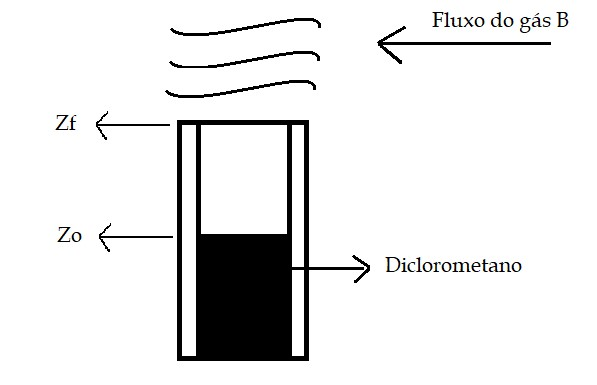
\includegraphics[scale=0.6,trim={0 0 0 0}]{figuras/ladeq/difusao/aparatoTeo}
		%\vspace{-20pt}
		\caption{Esquema da Célula de Arnold}
		\label{apaTeo}
	\end{center}
\end{figure}



\section{Considerações do modelo}



\begin{itemize}

\item Mistura binária;
\item Temperatura e pressão constantes;
\item Estado Pseudo-estacionário $\frac{DC_A}{dt}= 0$;
\item $D_{AB}$ não varia ao longo do processo difusivo;
\item Modelo de Fick é válido;
\item Difusão unidimensional (apenas o diclorometano se difunde);
\item Sistema homogêneo;
\item Não há reação química $r_A=0$;
\item O ar é insolúvel no diclorometano.

\end{itemize}

Desta forma, pelo modelo de Fick e aplicando a conservação de massa na fase gasosa, temos que:

Sabe-se que as moléculas se movem de forma aleatória ao longo do espaço disponível. Entretanto na aleatoriedade do movimento é possível observar um comportamento de conjunto que favorece um fluxo de partículas no sentido que sai da região de maior concentração para aa região com menor concentração. Dessa interpretação, surge o conceito básico de \emph{fluxo molar difusivo}, dado pela primeira lei de Fick: 

\begin{equation}\label{key}
J_{A}=-D_{A B} \nabla C_{A}
\end{equation}

Como no presente experimento, considera-se que a difusão ocorre apenas no sentido vertical, com orientação para cima, a lei assume a forma:

\newpage

%\begin{equation}\label{key}
%\mathrm{J}_{\mathrm{A}}=-\mathrm{D}_{\mathrm{AB}} \partial \mathrm{C}_{\mathrm{A}} \partial z
%\end{equation}

\begin{equation}\label{key}
\mathrm{J}_{\mathrm{A}}=-\mathrm{D}_{\mathrm{AB} } \dfrac{\partial \mathrm{C}_{\mathrm{A}}}{\partial z} 
\end{equation}


$D_{AB}$ - é a constante de proporcionalidade chamada coeficiente de difusão

Esse transporte de matéria causado pelo movimento das partículas pode também ser representado considerando a concentração das mesmas associadas à sua velocidade média, que pode ser escrita da forma: 


\begin{equation}\label{key}
\mathrm{J}_{\mathrm{A}}=\mathrm{C}_{\mathrm{A}}\left(\mathrm{v}_{\mathrm{A}, \mathrm{z}}-\mathrm{V}_{\mathrm{z}}\right)
\end{equation}


onde: 

\begin{itemize}
	\item $\mathrm{v}_{\mathrm{A}, \mathrm{z}}$: velocidade média de A na direção z.
	\item $V_{z}$: velocidade média da solução como um todo, também em z, dada para dois componentes por: 
	\begin{itemize}
		\item $V_{z}=\frac{1}{C}\left(C_{A} V_{A, z}-V_{z}\right)+C_{A} V_{z}=C_{A} V_{A, x}$
	\end{itemize}
\end{itemize}


O fluxo molar difusivo associado ao convectivo geram o fluxo molar total que é representado por:

\begin{equation}\label{key}
N_{A}=-C D_{A B} \frac{\partial Y _{A}}{\partial z}+Y_{A}\left(N_{A}+N_{B}\right)
\end{equation}

Tendo em vista que $N_{B} = 0$:

\begin{equation}\label{key}
N_{A}=-C D_{A B} \frac{\partial Y _{A}}{\partial z}+Y_{A} N_{A}
\end{equation}
\newpage

Que reescrita fica:

\begin{equation}\label{key}
N_{A}=\frac{C D _{A B}}{Z_{2}-Z_{1}} \ln \left(\frac{1-Y _{A 2}}{1-Y _{A 1}}\right), Z_{2}=Y_{A 2}=0
\end{equation}

Pela equação de balanço na interface:

\begin{equation}\label{key}
\frac{2 C _{A}}{\partial t}+\frac{2 N _{A}}{\partial z}=0 \operatorname{com} N_{A}=-C D_{A B} \frac{1}{1-Y _{A}} \frac{d Y _{A}}{d z}
\end{equation}

Realizando o balanço de massa na interface,

\begin{equation}\label{key}
\mathrm{N}_{\mathrm{A}}=\mathrm{C}_{\mathrm{A}}\left.\mathrm{v}_{\mathrm{A}}\right|_{z} \mapsto \mathrm{C}_{\mathrm{AL}} \frac{d L}{d t}
\end{equation}

Por fim, temos:

\begin{equation}\label{key}
N_{A}=C_{A L} \frac{d L}{d t}=\frac{C D_{AB}}{L} \ln \left(\frac{1}{Y _{A 1}}\right)=-C D_{A B} \ln \left(1-Y_{A 1}\right)
\end{equation}

Realizando a integral, encontra-se

\begin{equation}\label{key}
L^{2}-L_{0}^{2}=-2 \frac{\frac{C D _{A B}}{C_{A L}}} \ln \left(1-Y_{A 1}\right) t
\end{equation}

Por meio da obtenção do comportamento da altura ao longo do tempo, é possível realizar o cálculo de DAB. 
\\

\chapter{Determinação do Coeficiente de Difusão}


\section{Cálculo Teórico}

Foram usadas duas equações para o cálculo teórico do coeficiente de difusão.
A primeira foi a equação semi-empírica proposta por \citep{Fuller}. Foi reportado em literatura que a predição apresenta erros em torno de 7\% e pode ser usada tanto para pares de gases polares como apolares.


\begin{equation}\label{key}
D_{A B}=\frac{1.0 \times 10^{-9} T^{1.75}}{P\left[\left(\sum v\right)_{A}^{1 / 3}+\left(\sum v\right)_{B}^{1 / 3}\right]^{2}}\left(\frac{1}{M_{A}}+\frac{1}{M_{B}}\right)^{1 / 2}
\end{equation}


onde:

\begin{itemize}

\item T é a temperatura em K

\item P é a pressão em atm

\item $M_{A}$ e $M_{B}$ é a massa molar das substâncias,

\item $\Sigma_{v}$ é a soma dos volumes atômicos dos elementos de cada molécula (obtidos da tabela 2-2 do Hines e Maddox)

\end{itemize}

O valor calculado por Fuller foi de $1,07 \times 10^{-5} [\dfrac{m^{2}}{s}]$.

Uma segunda equação foi a de Chapman-Enskog, que é recomendada para pares de gases apolares. 

\begin{equation}\label{key}
D_{A B}=\frac{1.858 \times 10^{-27} T^{3 / 2}}{P \sigma_{A B}^{2} \Omega_{D}}\left(\frac{1}{M_{A}}+\frac{1}{M_{B}}\right)^{1 / 2}
\end{equation}

onde:

\begin{itemize}

\item $D_{AB}$ é a difusividade, $\dfrac{m^{2}}{s}$;
\item T é a temperatura absoluta, K;
\item M é a massa molecular, $\dfrac{kg}{kgmol}$;
\item P é a pressão absoluta, atm;
\item $\sigma_{AB}$ é o diâmetro de colisão, m;
\item $\Omega_{D}$ integral de colisão.

\end{itemize}



\begin{equation}\label{key}
\Omega_{D}=\left(44.54 T^{\sigma-4.909}+1.911 T^{\sigma-1.575}\right)^{0.10}
\end{equation}

Brokaw propôs uma correção no valor da integral de colisão ($\Omega_{D}$) considerando o momento de dipolo das moléculas, para calcular o coeficiente de difusão para pares de moléculas polares. No entanto, como neste caso temos uma molécula polar (diclorometano) e uma mistura apolar (ar) o fator $\delta_{A B}$ é 0, o que faz com que a integral de colisão para esse caso seja calculada da maneira prevista por Chapman e Enskog.

Correções de Brokaw:

\begin{itemize}
\item $\Omega_{D^{\sigma}}=\Omega_{D}+0.19 \delta_{A \beta}^{2} / T^{\circ}$

\item $\sigma_{A B^{\sigma}}=\left(\sigma_{A} \cdot \sigma_{B^{*}}\right)^{1 / 2}$

\item $\delta_{A B}=\left(\delta_{A} \delta_{B}\right)^{1 / 2}$

\item $\varepsilon_{A B^{\sigma}}=\left(\varepsilon_{A^{\sigma}} \varepsilon_{B^{\sigma}}\right)^{1 / 2}$

\item $\delta=\frac{1.94 \times 10^{3} \mu_{p}^{2}}{V_{b} T_{b}}$

\end{itemize}


\begin{figure}[H]
	\begin{center}
		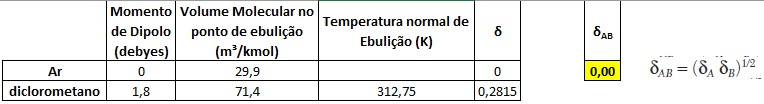
\includegraphics[scale=0.8,trim={0 0 0 0}]{figuras/ladeq/difusao/tab1}
		%\vspace{-20pt}
		\caption{Dados usados para o cálculo.}
		\label{tab1}
	\end{center}
\end{figure}


\begin{figure}[H]
	\begin{center}
		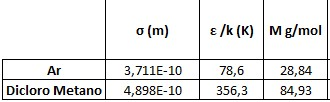
\includegraphics[scale=0.8,trim={0 0 0 0}]{figuras/ladeq/difusao/tab2}
		%\vspace{-20pt}
		\caption{Dados usados para o cálculo.}
		\label{tab2}
	\end{center}
\end{figure}


Dadas as considerações, o coeficiente de difusão calculado pela equação de Chapman-Enskog foi de $1,023 \times 10^{-5}  \dfrac{m^{2}}{s}$.

\chapter{Resultados e Discussão}

\section{Dados Experimentais}

Foi observado durante o experimento que a temperatura do banho não se manteve constante no valor ajustado no controlador de temperatura do equipamento. A temperatura foi ajustada para o valor de $28^{\circ} C$. A variação da temperatura marcada pelo controlador pode ser observada no gráfico da Figura \ref{temp}.


\begin{figure}[H]
	\begin{center}
		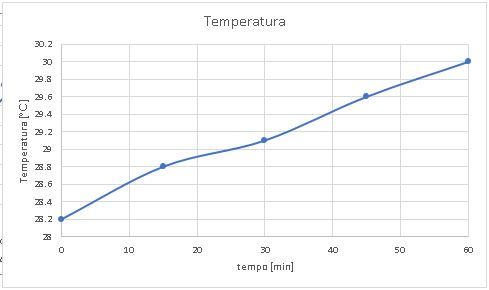
\includegraphics[scale=0.8,trim={0 0 0 0}]{figuras/ladeq/difusao/tempGraph}
		%\vspace{-20pt}
		\caption{Variação da temperatura ao longo do experimento.}
		\label{temp}
	\end{center}
\end{figure}

A principal variável de modelagem do experimento é a altura ou nível de diclorometano dentro da célula de Arnold. A dados coletados no experimento podem ser observados no gráfico da Figura \ref{diclo}.




\begin{figure}[H]
	\begin{center}
		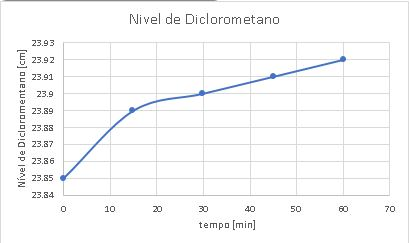
\includegraphics[scale=1,trim={0 0 0 0}]{figuras/ladeq/difusao/nivelDiclo}
		%\vspace{-20pt}
		\caption{Variação do nível de diclorometano com altura corrigida.}
		\label{diclo}
	\end{center}
\end{figure}

Para melhor visualização da variação do nível, calculou-se a variação do nível de diclorometano em relação ao nível inicial na célula de Arnold. Conforme podemos ver no gráfico da Figura \ref{delta} a variação total no nível foi menor do que o esperado e isso pode ter fonte de erros para os valores calculados. A pequena variação pode ser atribuída à algumas causas, como:

\begin{itemize}
	\item Quantidade de diclorometano inicial muito pequena;
	\item Contaminação do diclorometano.
\end{itemize}

Estas hipótese foram levantadas, pois a montagem do aparato e a preparação da carga de diclorometano foi realizada muito antes do início do experimento. Isso gerou algumas incertezas quanto a composição do líquido presente na célula de Arnold. A falta de diclorometano no estoque também impossibilitou o experimento com um nível inicial maior.

\begin{figure}[H]
	\begin{center}
		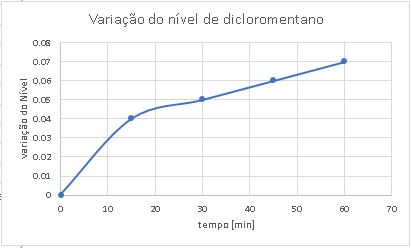
\includegraphics[scale=1,trim={0 0 0 0}]{figuras/ladeq/difusao/delta}
		%\vspace{-20pt}
		\caption{Variação do nível de diclorometano com altura corrigida.}
		\label{delta}
	\end{center}
\end{figure}


A partir dos dados experimentais foram então calculados os coeficientes de difusão para comparação com os dados encontrados na literatura.

\section{Determinação do coeficiente de difusão experimental}

Primeiramente é necessário calcular a pressão de saturação do diclorometano nas condições do experimento. Considerando a temperatura de $28 ^{\circ}$ C e pressão atmosférica de 1 atm.

Dados:

\begin{itemize}
	\item Temperatura: 303,15 [K];
	\item Pressão: $1,01325 \times 10^{5} [\mathrm{Pa}]$
\end{itemize}

\begin{equation}\label{key}
\ln P s a t=A-\frac{B}{T+C}
\end{equation}

O parâmetros utilizados e o valor calculado para a pressão de saturação pode ser observado na Tabela \ref{tab:sat}

\begin{table}[H]
	\centering
	\begin{tabular}{|l|l|l|}
		\hline
		\multicolumn{3}{|c|}{\textbf{Cálculo de Psat}} \\ \hline
		\textbf{T} & 28 & °C \\ \hline
		\textbf{A} & 13.9891 &  \\ \hline
		\textbf{B} & 2463.93 &  \\ \hline
		\textbf{C} & 223.24 &  \\ \hline
		\textbf{ln Psat} & 4.18 &  \\ \hline
		\textbf{Psat} & 65.50 & kPa \\ \hline
	\end{tabular}
	\caption{Cálculo da pressão de Saturação}
	\label{tab:sat}
\end{table}

A partir da pressão de saturação foram calculados os valores de concentração de diclorometano próxima a interface líquido-ar. Foram utilizadas as seguintes fórmulas:

\begin{equation}\label{key}
y_{A i}=\frac{P_{A}^{SAT}(T)}{P}
\end{equation}

\begin{equation}\label{key}
C=\frac{P}{R T}
\end{equation}

A concentração de diclorometano na fase líquida poder ser calculada por:

\begin{equation}\label{key}
C_{A, L}=\frac{\rho_{A, L}}{M_{A}}
\end{equation}

E finalmente o cálculo do coeficiente de difusão é obtido através da equação:


\begin{equation}\label{key}
D_{A B}=\frac{\text {coef.angular} \cdot C_{A L}}{-2 \cdot C \cdot \ln \left(1-y_{A i}\right)}
\end{equation}

O coeficiente angular é dado pela seguinte equação:

\begin{equation}\label{key}
\text {coef.angular}=\frac{L^{2}-L_{0}^{2}}{t}
\end{equation}

Ou seja, o coeficiente angular foi obtido através da regressão dos dados experimentais.


\section{Ajuste linear para altura corrigida}


Na Figura \ref{linear} podemos observar a reta obtida através dos dados de altura no nível de diclorometano corrigida com a altura do bocal da célula de Arnold.

\begin{figure}[H]
	\begin{center}
		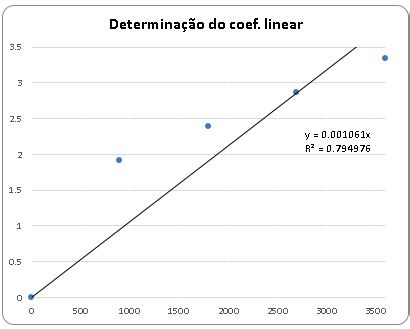
\includegraphics[scale=1,trim={0 0 0 0}]{figuras/ladeq/difusao/linear00}
		%\vspace{-20pt}
		\caption{Regressão dos dados experimentais para obtenção do coeficiente angular.}
		\label{linear}
	\end{center}
\end{figure}

A Tabela \ref{tab:dif} apresenta os cálculos para a obtenção do coeficiente de difusão experimental.


\begin{table}[H]
		\centering
	\begin{tabular}{|l|l|l|}
		\hline
		\multicolumn{3}{|c|}{\textbf{Cálculos}} \\ \hline
		Psat & 65498.23 & Pa \\ \hline
		$y_{A1}$ & 0.6464 &  \\ \hline
		C & 40.47 & mol/m³ \\ \hline
		$C _{AL}$ & 15659.96 & mol/m³ \\ \hline
		\begin{tabular}[c]{@{}l@{}}Coeficiente exp\end{tabular} & 1.06E-03 &  \\ \hline
		\multicolumn{1}{|c|}{\multirow{2}{*}{$D_{AB}$}} & 1.98E-01 & cm²/s \\ \cline{2-3} 
		\multicolumn{1}{|c|}{} & 1.98E-05 & m²/s \\ \hline
	\end{tabular}
	\caption{Cálculo do coeficiente de difusão.}
	\label{tab:dif}
\end{table}

\section{Ajuste linear para altura medida}

Na Figura \ref{linear2} podemos observar a reta obtida através dos dados de altura no nível de diclorometano sem a correção com a altura do bocal da célula de Arnold.

\begin{figure}[H]
	\begin{center}
		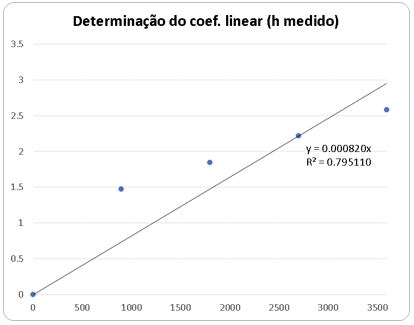
\includegraphics[scale=1,trim={0 0 0 0}]{figuras/ladeq/difusao/linear002}
		%\vspace{-20pt}
		\caption{Regressão dos dados experimentais para obtenção do coeficiente angular.}
		\label{linear2}
	\end{center}
\end{figure}

A Tabela \ref{tab:dif2} apresenta os cálculos para a obtenção do coeficiente de difusão experimental.


\begin{table}[H]
	\centering
	\begin{tabular}{|l|l|l|}
		\hline
		\multicolumn{3}{|c|}{\textbf{Cálculos}} \\ \hline
		Psat & 65498.23 & Pa \\ \hline
		$y_{A1}$ & 0.6464 &  \\ \hline
		C & 40.47 & mol/m³ \\ \hline
		$C _{AL}$ & 15659.96 & mol/m³ \\ \hline
		\begin{tabular}[c]{@{}l@{}}Coeficiente exp\end{tabular} & 8.20E-04 &  \\ \hline
		\multicolumn{1}{|c|}{\multirow{2}{*}{$D_{AB}$}} & 1.53E-01 & $cm^{2}/s$ \\ \cline{2-3} 
		\multicolumn{1}{|c|}{} & 1.53E-05 & $m^{2}/s$ \\ \hline
	\end{tabular}
	\caption{Cálculo do coeficiente de difusão.}
	\label{tab:dif2}
\end{table}


\chapter{Análise dos Resultados}


Comparando-se os valores de $D_{AB}$ obtidos experimentalmente, percebemos que quando desconsideramos a altura entre o papel milimetrado e a abertura do tubo, o valor do coeficiente de difusão obtido é menor do que quando considerado $(1,98 \times 10^{-5} m^{2}/s$ e $1,53 \times 10^{-5} m^{2}/s$, respectivamente), o que pode ser explicado pelo fato de estarmos subestimando o caminho difusivo percorrido pelo gás, então o valor do coeficiente de difusão deve ser menor. Já ao comparar os valores de $D_{AB}$ obtidos experimentalmente com os valores teóricos, o valor calculado (considerando a altura) foi maior do que os valores teóricos (\citep{Fuller}: $ 07 \times 10^{-5} m^{2}/s; Chapman-Enskog: 1,023 \times 10^{-5} m^{2}/s$), algo inesperado pelo menos de acordo com o objetivo da prática, em que os valores deveriam ser próximos dos valores teóricos, com porcentagem de erro considerável. Mesmo assim, o resultado e as condições da prática confirmam o valor diferente dos valores teóricos, cuja informação pôde ser concretizada com o valor do $R^{2}$ gerado no gráfico do cálculo do coeficiente de difusão ($R^{2}$ = 0,795110, o qual deveria ser próximo de 1,0).

Diversos motivos podem ter sido responsáveis por essa diferença no valor do coeficiente de difusão, sendo possível citar, por exemplo, erros na leitura das alturas do diclorometano ao longo do tempo, visto que tal leitura foi realizada individualmente por cada componente do grupo, para depois obterem-se os respectivos valores médios, sendo que tais leituras deveriam ter sido tomadas de forma rápida, já que estavam variando constantemente, sem contar que a escala utilizada em papel milimetrado era imprecisa. Além disso, como a temperatura ao longo do experimento não se manteve constante, isso deve ter gerado erros na medição da mesma por parte do aparelho, não esquecendo das hipóteses e aproximações realizadas nos cálculos de $D_{AB}$, que podem gerar outros pequenos erros. Contudo, a hipótese mais plausível e considerável para o experimento foi o fato de que o diclorometano pode ter sido contaminado, o que impossibilitou a credibilidade e, consequentemente, uma análise adequada do experimento, mesmo o valor do coeficiente de difusão experimental obtido estando dentro da faixa de ordem de grandeza esperada para coeficientes de difusão de gases ($10^{-5}$ a $10^{-6} m^{2}/s$).
\\

\chapter{Conclusão}

Através do experimento realizado, foi possível observar o fenômeno de difusão do diclorometano em ar, permitindo obter dados para plotar um gráfico que resultou no cálculo do coeficiente de difusão mássica do conjunto de componentes. O valor encontrado deve ser desconsiderado, mesmo se encontrando dentro da faixa de valores de coeficientes de difusão para gases, visto que houve uma contaminação do diclorometano, impossibilitando a análise e devida comparação do resultado com os modelos teóricos propostos e, por conta disso, o experimento deve ser repetido.

%\chapter{Objetivo}

Avaliar a resposta no tempo de um sistema de dois tanques em série após uma perturbação degrau na temperatura do primeiro tanque e comparar os resultados obtidos empiricamente com os previstos pelos modelos fenomenológicos.


\chapter{Descrição da prática}

\section{Equipamentos e instrumentação utilizados}

\begin{itemize}
\item Dois termopares (um em cada tanque);
\item Dois tanques com água, em série, com agitação e volume constante;
\item Bomba hidráulica;
\item Resistor (125 V e 9 A);
\item Mangueiras e uma válvula (na entrada do primeiro tanque);
\item Sistema de Controle - Software iFix.
\end{itemize}

\begin{figure}[H]
	\begin{center}
		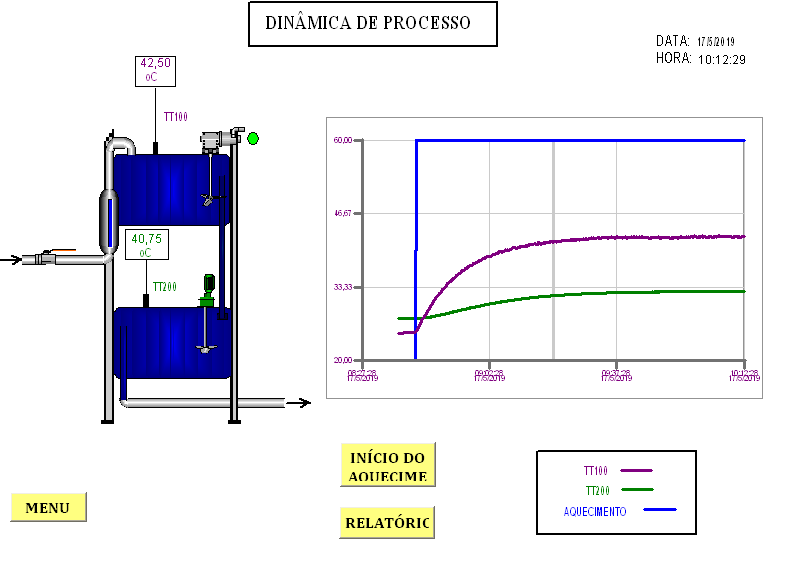
\includegraphics[scale=.8, trim={0 0 0 0}]{figuras/ladeq/dina/ft2}
		%\vspace{-20pt}
		\caption{Tanques abertos, em série, com agitação e sistema de aquecimento no primeiro tanque.}
		\label{aparato}
	\end{center}
\end{figure}

\section{Procedimento experimental}

Dois tanques em série possuem a mesma vazão de entrada e saída e estão com aproximadamente a mesma temperatura no início do processo ($ T1 = 24,82 \  ^{\circ}C \  e \ T2 =24,62 \ ^{\circ}C) $; Em determinado momento, aciona-se o aquecedor acoplado ao primeiro tanque, promovendo uma perturbação degrau no sistema que o induz a um comportamento transiente durante determinado tempo até que um novo estado estacionário seja obtido. Tal momento, de início do aquecimento, é registrado na figura 2 pela linha azul no gráfico. 

A perturbação é monitorada por dois sensores que, conectados a um computador, acompanham a variação da temperatura nos dois tanques. No iFix (software utilizado para acompanhamento do processo), as curvas TT100 (curva roxa) e TT200 (curva verde) representam as temperaturas dos tanques 1 e 2, respectivamente, ao longo do tempo. Pode-se observar que após certo período, o novo valor de temperatura foi estabilizado em $ 42,5 \ ^{\circ}C $ no tanque 1 e $ 40,75 \ ^{\circ}C  $no tanque dois. A ligeira diferença se deve ao fato do tanque 1 receber diretamente o aquecimento.


\begin{figure}[H]
	\begin{center}
		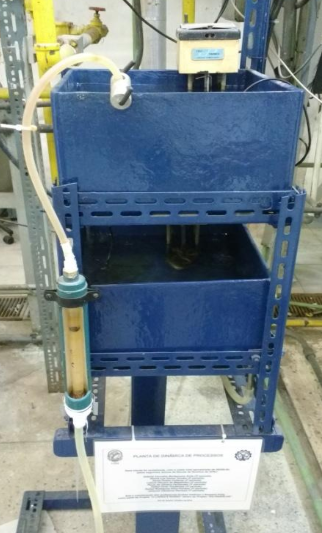
\includegraphics[scale=.8, trim={0 0 0 0}]{figuras/ladeq/dina/ft1}
		%\vspace{-20pt}
		\caption{Monitoramento da prática obtida através do software iFix.}
		\label{iFix}
	\end{center}
\end{figure}


\chapter{Cálculos}


Pela Tabela \ref{tab1} podemos observar quanto tempo levou, após acionarmos o aquecimento, para que cada tanque iniciasse seu aquecimento. Esse tempo entre o acionamento e o inicio dos efeitos na variável controlada foi estimado como o tempo morto do sistema. 

\begin{table}[H]
	\centering
	\begin{tabular}{|c|c|c|}
		\hline
		\textbf{t(s)}                 & \textbf{T2}                   & \textbf{T1}                   \\ \hline
		0.00                          & 24.88                         & 25.15                         \\ \hline
		...                           & ...                           & ...                           \\ \hline
		\cellcolor[HTML]{F8FF00}3.00  & 24.88                         & \cellcolor[HTML]{F8FF00}25.15 \\ \hline
		4.00                          & 24.82                         & 25.21                         \\ \hline
		...                           & ..                            & ..                            \\ \hline
		\cellcolor[HTML]{FCFF2F}50.00 & \cellcolor[HTML]{FCFF2F}24.88 & 26.19                         \\ \hline
		51.00                         & 24.95                         & 26.25                         \\ \hline
	\end{tabular}
\caption{Valores definidos como constantes de tempo morto para T1 e T2.}
\label{tab1}
\end{table}

Portanto o tempo morto para o tanque 1, ou seja, $ t_{01} $ é igual a 3 segundos. Já o tempo morto para o segundo sistema, $ t_{02} $ é igual a 50 segundos.

Foi determinada então a amplitude da perturbação. Durante o experimento foram coletados dados do aquecedor elétrico utilizando um multímetro, foi medida a corrente e a tensão do aquecedor. Com esses valores foi possível calcular a potência do aquecedor com base na Equação \ref{pot}:

\begin{equation}\label{pot}
\text{Potência}= \text{Tensão} \cdot \text{Corrente} = 125 V \cdot 9 A=1125 W
\end{equation}

\section{Cálculo das constantes para o Tanque 1}

Forma geral da função de transferência para um sistema de primeira ordem exemplificado pela Equação \ref{1ordem}.
\begin{equation}\label{1ordem}
G_{1}(s)=\frac{k_{1}}{\tau_{1} s+1} e^{-t_{01} s}
\end{equation}

Cálculo dos parâmetros da função de transferência

\begin{equation}\label{key}
k 1=\frac{T_{1}-T_{0}}{\text {Degrau}}=\frac{\Delta T}{\text {Degrau}}
\end{equation}

\begin{equation}\label{key}
T_{1}\left(\tau_{1}\right)=0,632 * P * k_{1}
\end{equation}

Primeira ordem em função do tempo:

\begin{equation}\label{key}
T_{1}(t)=A k_{1}\left(1-\exp \exp \left(-\frac{\left(t-t_{01}\right)}{\tau_{1}}\right)\right)
\end{equation}

Calculando com os valores obtidos durante o experimento

\begin{equation}\label{key}
k 1=\frac{42,50-25,15}{1125}=0,01543 \ \frac{^{\circ} C}{W}
\end{equation}

\begin{equation}\label{key}
\left[T_{1}\left(\tau_{1}\right)=0,632 \cdot P \cdot k_{1}=0,632 \cdot 1125 \cdot 0,01543=10,97073^{\circ} C\right.
\end{equation}


De posse dos valores obtidos no experimento, a temperatura do Tanque 1 estava em T1 = 25,15 +10,97 = 36,12073 em t = 749 segundos. Considerando o tempo morto, teremos 752 segundos.]

Chegamos então a seguinte função de transferência:


\begin{equation}\label{key}
G_{1}(s)=\frac{0,01543}{752 s+1} e^{-3 s}
\end{equation}


\begin{equation}\label{key}
T_{1}(t)=17,36\left(1-\exp \exp \left(-\frac{(t-3)}{749}\right)\right)
\end{equation}
 
Plotar o experimental juntamente do calculado:

\begin{figure}[H]
	\begin{center}
		\includegraphics[scale=.5, trim={0 0 0 0}]{figuras/ladeq/dina/graph1}
		%\vspace{-20pt}
		\caption{Dados experimentais e dados obtidos da função de transferência em variável desvio.}
		\label{iFix}
	\end{center}
\end{figure}


\section{Cálculo das constantes para o Tanque 2}

Considerado um sistema de segunda ordem já que existiam dois sistemas de primeira ordem em série:

\begin{equation}\label{key}
G_{2}(s)=\frac{k_{2}}{\left(\tau_{21} s+1\right)\left(\tau_{22} s+1\right)} e^{-t_{02} s}
\end{equation}

Outra forma de se representar um sistema de segunda ordem é dado pela Equação \ref{2ordem}

\begin{equation}\label{2ordem}
G_{2}(s)=\frac{k_{2}}{\tau^{2} s^{2}+2 \xi \tau s+1} e^{-t_{02} s}
\end{equation}


Onde:

\begin{itemize}
	\item $ 2 \xi \tau=\tau_{21}+\tau_{22} $;
	\item $ \tau^{2}=\tau_{21} * \tau_{22} $.
\end{itemize}


Cálculo dos parâmetros da função de transferência:
\begin{equation}\label{key}
k 2=\frac{T_{2}-T_{0}}{D e g r a u}=\frac{\Delta T}{D e g r a u}
\end{equation}

O cálculo do ganho estático pela mesma Equação utilizada para o Tanque 1.

\begin{equation}\label{key}
k 2=\frac{40,81-24,88}{1125}=0.01416 \frac{^{\circ} C}{W}
\end{equation}

Quanto as constantes do comportamento dinâmico do tanque 2, foram determinadas da seguinte forma:

\begin{equation}\label{key}
T_{2}\left(\tau_{2}=0,73\right)=0,73 \cdot P \cdot k_{2}=0,73 \cdot 1125 \cdot 0.01416=11,9475 \ ^{\circ} C
\end{equation}

O tempo correspondente ao valor de temperatura $ T_2= 24,88 + 11,95 = 36,83 \ ^{\circ}C  $ foi de 1848 segundos. Descontando o tempo morto de 50 segundos teremos t = 1798 segundos. Com a metade deste tempo e somando o tempo morto, determinou-se a resposta correspondente do sistema,$ T_{2}\left(\frac{t_{3336}}{2}+t_{02}\right)=T_{s}=T(t=949 s)=31.38-24.88=6,50 \ ^{\circ} C . $Assim, resolveu-se o seguinte sistema:


\begin{equation}\label{key}
\left\{\begin{array}{c}{t_{73\%}=1,3\left(\tau_{21}+\tau_{22}\right)} \\ {\frac{T_{s}}{A k_{2}}=\frac{\tau_{22}}{\tau_{21}}}\end{array}\right. \rightarrow \left\{\begin{array}{c}{\tau_{21}=\frac{t_{73 \%}}{1,3\left(1+\frac{T_{s}}{P k_{2}}\right)}=1009,59 \mathrm{s}} \\ {\tau_{22}=\frac{T_{s}}{P k_{2}} \tau_{21}=411,95 \mathrm{s}}\end{array}\right.
\end{equation}

Portando:

\begin{itemize}
\item $ \tau=\sqrt{\tau_{21} \cdot \tau_{22}}=\sqrt{1009,59 \cdot 411,95}=644,90 $
\item $ \xi=\frac{\tau_{21}+\tau_{22}}{2 \cdot \tau}=\frac{1009,59+411,95}{2 \cdot 644,90}=1,10 $
\end{itemize}


Com base no valor obtido para a constante de amortecimento do sistema, $ \xi $, podemos classificá-lo como um sistema superamortecido sem oscilação. O que de fato foi observado na resposta da temperatura do Tanque 2.

\newpage

Assim, função de transferência obtida é dada por:

\begin{equation}\label{key}
G_{2}(s)=\frac{0,01421}{(1009,59+1)(411,95 s+1)} e^{-50 s}
\end{equation}

Ou: 

\begin{equation}\label{key}
G_{2}(s)=\frac{k_{2}}{640,99^{2} s^{2}+2 \cdot 1,1 \cdot 640,99 s+1} e^{-50 s}
\end{equation}

Em função do tempo, o sistema de segunda ordem pode ser descrito como:

\begin{equation}\label{key}
T_{2}(t)=P k_{2}\left(1-\frac{\left(-\frac{\left(t-t_{02}\right)}{\tau_{21}}\right)-\left(-\frac{\left(t-t_{02}\right)}{\tau_{22}}\right)}{\tau_{21}-\tau_{22}}\right)
\end{equation}


A função dependente do tempo é dada por:


\begin{equation}\label{key}
T_{2}(t)=15.93\left(1-\frac{1009,59 \exp \exp \left(-\frac{(t-50)}{1009,59}\right)-411,95 \exp \exp \left(-\frac{(t-50)}{411,95}\right)}{813.81}\right)
\end{equation}


\begin{figure}[H]
	\begin{center}
		\includegraphics[scale=.5, trim={0 0 0 0}]{figuras/ladeq/dina/graph2}
		%\vspace{-20pt}
		\caption{Dados experimentais e dados obtidos da função de transferência em variável desvio.}
		\label{iFix}
	\end{center}
\end{figure}

Abaixo na Figura \ref{dois} é possível comparar o diferente comportamento dinâmico dos dois tanques. Em ambos os casos as curvas obtidas pela  metodologia empírica de determinação da função de transferência se correlacionaram muito fortemente com as previstas fenomenologicamente.




\begin{figure}[H]
	\begin{center}
		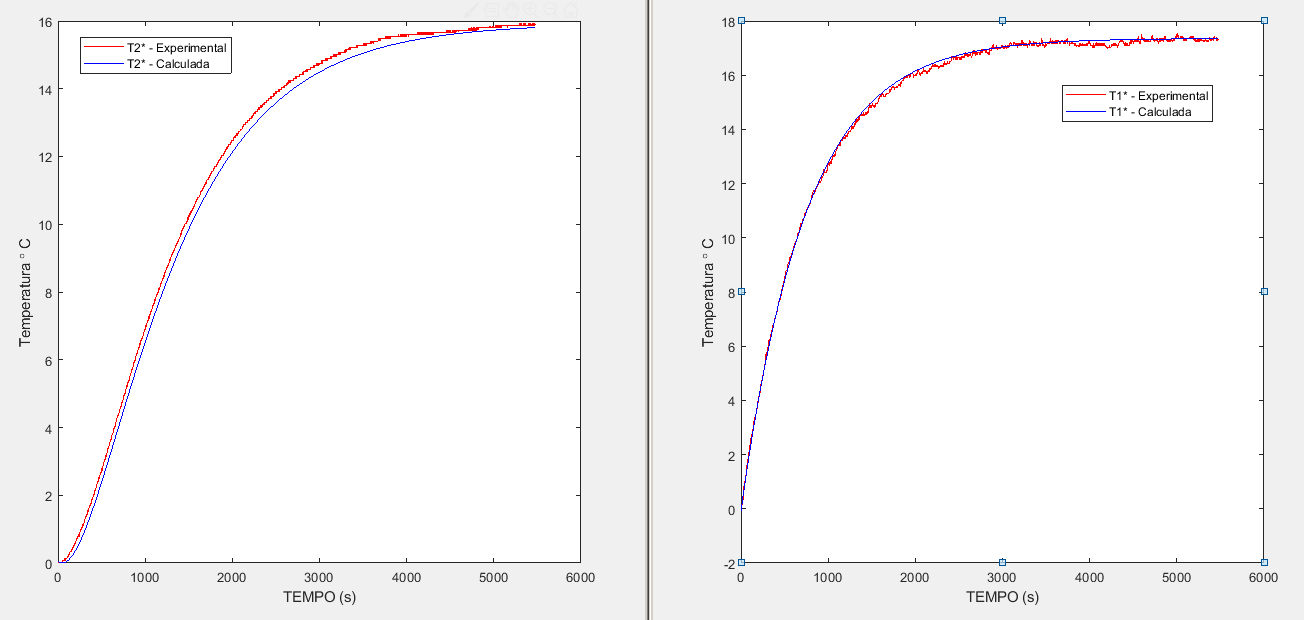
\includegraphics[scale=.5, trim={0 0 0 0}]{figuras/ladeq/dina/graph3}
		%\vspace{-20pt}
		\caption{Dados experimentais e dados obtidos para as temperatura dos Tanques 1 e 2.}
		\label{dois}
	\end{center}
\end{figure}


\chapter{ Conclusões}

De acordo com o que foi observado por meio dos dados obtidos na prática, pode-se concluir que as premissas adotadas de comportamento, de primeira ordem para o primeiro tanque, e de segunda ordem para o segundo tanque, num sistema de tanques agitados em série se mostrou válida. Ambas as curvas obtidas pelo modelo fenomenológico mostraram forte correlação com as os dados empíricos. No primeiro tanque o tempo morto foi pequeno, de apenas 3 segundos, indicando uma boa agitação, visto que a variação de temperatura foi prontamente detectada pelo termopar. Já no segundo tanque, houve um tempo morto maior, isto é de 50 segundos, uma vez que a variação de temperatura no segundo tanque dependia do aumento de temperatura do primeiro. 

O valor do coeficiente de amortecimento encontrado para o segundo tanque indica comportamento superamortecido (>1), o que pode ser corroborado pela curva que não apresentou caráter oscilatório como resposta à perturbação degrau.













%\chapter{Fundamentação Teórica}

Em uma destilação batelada a medida que o tempo passa, o liquido do vaporizador fica mais pobre no componente mais volátil e mais rico no componente menos volátil por meio de sucessivas condensações e vaporizações que ocorrem dentro da coluna, especialmente na zona de recheio.

\subsection{Hipóteses adotadas:}

\begin{itemize}
	\item Abordagem simplificada, admitindo simplificações do Método McCabe-Thiele;
	\item Retenções de material nos pratos da coluno (Hold up's) foram desprezadas;
	\item Taxas de vaporização constante;
	\item Equilíbrio Líquido Vapor entre o líquido no vaporizador e o vapor gerado no mesmo instante.
\end{itemize}


\subsection{Parâmetros}

\begin{itemize}
	\item \emph{t}: tempo;
	\item \emph{B(t)}: número de moles de líquido no vaporizador no instante t
	\item \emph{$B_{0}$}: valor de B(t) no instante t=0;
	\item \emph{$X_{B}(t)$}: fração molar do componente no instante t no vaporizador;
	\item \emph{$X_{B0}$}: fração molar do componente no instante t=0 no vaporizador;
	\item \emph{ D(t): }Vazão do destilado no instante t;
	\item \emph{$X_{D}(t)$}: fração molar do destilado no instante t;
	\item \emph{$X_{P}(t)$}: fração média do componente no tanque de produto no instante t (acumulado até o tempo t).
%	\item \emph{}
%	\item \emph{}
\end{itemize}


\subsection{Modelagem Matemática}


\begin{figure}[H]
	\begin{center}
		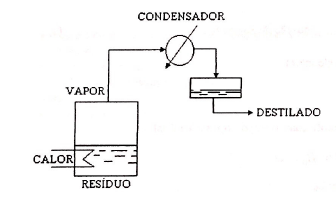
\includegraphics[scale=0.7,trim={0cm -9 0 0}]{figuras/ladeq/destil/modelo}
		\vspace{-20pt}
		\caption{Modelo de destilador de batelada.}
		\label{ladeq/batelada}
	\end{center}
\end{figure}

Equações:


\begin{equation}\label{eq1}
\frac{\mathrm{d} }{\mathrm{d} t}(Bx_{B}) = -Dx_{D}
\end{equation}

\begin{equation}\label{eq2}
x_{B} \frac{\mathrm{d} }{\mathrm{d} t}B + B\frac{\mathrm{d} }{\mathrm{d} t}x_{B} = -Dx_{D}
\end{equation}

\begin{equation}\label{eq3}
x_{B} \mathrm{d} B + B \mathrm{d} x_{B} = -Dx_{D}\mathrm{d}t
\end{equation}

\begin{equation}\label{eq4}
D = -\frac{\mathrm{d} }{\mathrm{d} t}B \rightarrow D \mathrm{d} t = -\mathrm{d} B
\end{equation}

Substituindo \ref{eq4} em \ref{eq3}:

\begin{equation}\label{eq5}
x_{B}\mathrm{d} B + B \mathrm{d} x_{B} = x_{D} \mathrm{d}B
\end{equation}

Rearranjando a equação \ref{eq5}
\begin{equation}\label{eq6}
(x_{B} - x_{D}) \mathrm{d}B = - B\mathrm{d} x_{B}
\end{equation}

\begin{equation}\label{eq7}
(x_{D} - x_{B}) \mathrm{d}B = B\mathrm{d} x_{B}
\end{equation}

Separando as variáveis:

\begin{equation}\label{eq8}
\frac{\mathrm{d} B}{B} = \frac{\mathrm{d} x_{B}}{(x_{D} - x_{B})}
\end{equation}

Fazendo a integral do tempo 0 até um determinado tempo t:

\begin{equation}\label{eq9}
\int_{B_{0}}^{B} \frac{\mathrm{d}B}{B} = \int_{B_{0}}^{B} \frac{\mathrm{d}x_{B}}{(x_{D} - x_{B})}
\end{equation}


Equação \ref{eq10} também é conhecida como Equação de Rayleigh:

\begin{equation}\label{eq10}
\ln (\frac{B}{B_{0}}) = \int_{x_{B0}}^{x_{B}} \frac{\mathrm{d}x_{B}}{(x_{D} - x_{B})}
\end{equation}

Se integramos o balanço global (\ref{eq4}):

\begin{equation}\label{eq11}
\int_{0}^{t} D \mathrm{d}t = \int_{B_{0}}^{B} -\mathrm{d}B
\end{equation}

Sabendo-se que D é constante com o tempo, suposição inicial:

\begin{equation}\label{eq12}
-D t = B - B_{0} \rightarrow B = B_{0} - Dt
\end{equation}

Divide-se a equação \ref{eq11} por $B_{0}$:

\begin{equation}\label{eq13}
\frac{B}{B_{0}} = 1 - \frac{Dt}{B_{0}}
\end{equation}


Tempo de Batelada:

\begin{equation}\label{eq14}
t = \frac{B_{0}}{D} \left \{ 1 - \exp \left ( \int_{x_{B0}}^{x_{B}}  \frac{\mathrm{d} x_{B}}{(x_{D}-x_{B})} \right ) \right \}
\end{equation}

Balanço de massa por componente no instante t:

\begin{equation}\label{eq15}
B_{0} x_{B0} = B(t)x_{B}(t) + (B_{0} - B(t))x_{p}t
\end{equation}

\begin{equation}\label{eq16}
x_{p}(t) = \frac{ x_{B0} - \frac{B(t)}{B_{0}} x_{B}(t) }{t - \frac{B(t)}{B_{0}}}
\end{equation}

\begin{equation}\label{eq17}
x_{p}(t) \frac{ x_{B0} - x_{B} \exp \int_{x_{B0}}^{x_{B}} \frac{\mathrm{d} x_{B}}{(x_{D}(t) - x_{B}(t))}}{1 -  \exp \int_{x_{B0}}^{x_{B}} \frac{\mathrm{d} x_{B}}{(x_{D}(t) - x_{B}(t))}}
\end{equation}







%\chapter{Introdução}



\chapter{Apresentação das equações utilizadas}

\section{Filtração}


Para uma filtração sólido-líquido com formação de torta e considerando a torta como um meio poroso, aplica-se a equação do movimento para a torta:

%\begin{tikzpicture}
%\draw (0,0) node{$\displaystyle{
%		\mathcal{L} \lbrace f(t)\rbrace = \int_{t=0}^\infty e^{-st} f(t)\,dt}$};
%\end{tikzpicture}


\begin{equation}\label{key}
\rho\left[\varepsilon \frac{\partial \frac{q}{\varepsilon}}{\partial t}+\nabla\left(\frac{q}{\varepsilon}\right) q\right]=-\nabla P+\nabla \tau-m+\rho g
\end{equation}


onde:

\begin{itemize}

\item $\rho$ = densidade
\item $\varepsilon$ = porosidade da torta
\item q = velocidade superficial
\item P = pressão do sistema
\item $\tau$ = parâmetro proveniente de forças viscosas
\item g = aceleração da gravidade
\item m = massa de sólidos na torta

\end{itemize}

Suposições:

\begin{itemize}
\item Sem forças de campo;
\item Estado estacionário;
\item $\mathrm{\nabla\tau}= 0$ (sem interação viscosa);
\item Meio poroso isotrópico (k = cte.);
\item Escoamento a baixas velocidades ($Re_{MP}<1,0$)
\item Fluído;
\item Meio poroso rígido ($\varepsilon$ = cte.);
\item Meio poroso estacionário;
\item Escoamento isotérmico e incompressível ($\rho$=cte.);
\item Unidimensional e horizontal.
\end{itemize}

Então:

\begin{equation}\label{key}
\mathrm{m}=-\nabla P
\end{equation}

Com equação do movimento e a de  Darcy:

\begin{equation}\label{key}
\frac{d P}{d x}=\frac{\mu}{k} q
\end{equation}


E utilizando a definição de porosidade:

\begin{equation}\label{key}
\mathrm{dM}=\rho_{s}(1-\varepsilon) A d x
\end{equation}

Onde:

\begin{itemize}
\item $\mu$ = viscosidade do fluido;
\item A = área de filtração;
\item $\rho_{s}$ = densidade do sólido.
\end{itemize}

Fazendo as devidas substituições: e considerando PL = constante:

\begin{equation}\label{key}
d(P L-P)=\left(\frac{\mu q}{k \rho_{s}(1-\varepsilon) A}\right) d M
\end{equation}

A resistividade da torta ($\alpha$):

\begin{equation}\label{key}
\alpha=\frac{1}{k \rho_{s}(1-\varepsilon)}
\end{equation}

Logo,

\begin{equation}\label{key}
\mathrm{d}(\mathrm{PL}-\mathrm{P})=\left(\frac{\mu q a}{A}\right) d M
\end{equation}


\section{Dimensionamento Industrial}


Para o escalonamento de um filtro piloto para um filtro industrial consideramos que ambos operam com a mesma suspensão, a mesma queda de pressão e sob a mesma temperatura. Utilizando o subscrito ‘P’ para Piloto e ‘I’ para Industrial, temos as Equações \ref{DI1} e \ref{DI2} :

\begin{equation}\label{DI1}
V_{t P}=\frac{A_{P}}{2} e_{P}
\end{equation}

\begin{equation}\label{DI2}
V_{t I}=\frac{A_{I}}{2} e_{I}
\end{equation}


Em que, Vt é o volume da torta e  “e” a espessura do quadro. Considerando que o volume de torta é proporcional ao volume de filtrado (V) e combinando \ref{DI1}, \ref{DI2} à equação de trabalho, temos as Equações \ref{DI3} e \ref{DI4} :

\begin{equation}\label{DI3}
\frac{t_{P}}{t_{I}}=\frac{\left(\frac{V_{P}}{A_{P}}\right)^{2}}{\left(\frac{V_{I}}{A_{I}}\right)^{2}}
\end{equation}

\begin{equation}\label{DI4}
t_{I}=t_{P}\left(\frac{e_{I}}{e_{P}}\right)^{2}
\end{equation}


Com o tempo total de filtração na escala piloto, obtém-se o tempo total de filtração na escala industrial pela equação 13. Sabendo que o volume de filtrado industrial pode ser determinado pela Equação \ref{DI5}, da Equação \ref{DI3} calcula-se a área total de filtração industrial.

\begin{equation}\label{DI5}
V_{I}=P_{t} \cdot T_{I}
\end{equation}

Em que P é a vazão de produção da unidade industrial.
A vazão de produção de filtrado pode ser calculada como sendo a razão entre o volume de filtrado e o tempo total do ciclo de operação, incluindo o tempo de filtração , o tempo de lavagem dos quadros  e o tempo de montagem dos quadros  para a próxima operação, de acordo com a Equação \ref{DI6}. 

\begin{equation}\label{DI6}
P=\frac{V}{t_{f i l t}+t_{l a v}+t_{m o n t}}
\end{equation}


\chapter{Materiais e Métodos}

\section{Materiais}

\begin{itemize}

\item Suspensão de carbonato de cálcio;
\item Três vidros de relógio numerados;
\item Três becher numerados;
\item Duas provetas graduadas de 2L;
\item Um bastão de vidro;
\item Cronômetro (foi utilizado o cronômetro do celular de um dos integrantes do grupo);
\item Régua;
\item Espátula;
\item Filtro prensa (formado por dois quadros sem recheio, três placas rugosas e dois meios filtrantes);
\item Balança digital;
\item Estufa.


\end{itemize}

\section{Métodos}

Os bécher e vidros de relógio foram pesados e enumerados. Foram medidas as dimensões do quadro do filtro prensa com o auxilio de uma régua. 

O filtro prensa foi montado utilizando dois meios filtrantes. Estes foram umedecidos previamente para minimizar vazamentos. O filtro prensa utiliza dois quadros vazados que servem de suporte para os meios filtrantes e três placas rugosas. Durante a montagem do filtro prensa é realizada sobre o trilho do equipamento com placas e quadros intercalados de forme que duas placas fiquem nas extremidades. Foi verificada sistematicamente com uso de uma caneta se os furos de placas e quadros coincidem para que a suspensão possa para por todo o circuito do filtro-prensa. Após a verificação do ajuste do filtro, apertou-se o parafuso que mantem os quadros unidos e vedados contra o vazamento.

A solução de carbonato de cálcio presente no tanque de alimentação foi homogeneizada com auxílio de um bastão de vidro. \emph{Três amostras foram retiradas da suspensão} e pesadas nos bécher previamente pesados e identificados. Essa amostras foram então encaminhadas para uma estufa \emph{desligada durante cinco dias. No quinto dia a estufa foi ligada e. no sexto dia, as amostras secas foram pesadas novamente.}
 
Antes do início da filtração as provetas foram posicionadas de forma a coletar a solução filtrada e facilitar a troca rápida quando a primeira proveta chegar ao nível máximo. Com o tanque de alimentação já em recirculação, foi aberta a válvula a montante do filtro-prensa.

Com auxilo de provetas, o filtrado foi coletado. Durante este processo foram realizadas a marcação de volume filtrado em relação ao tempo de filtração. Para a marcação do tempo foi utilizado cronometro de celular operado por um dos alunos e com avisos sonoros dos alunos que operavam a coleta do filtrado na proveta.

A vazão de filtrado diminuiu durante a filtração e o experimento foi finalizado quando esta vazão ficou próxima de nula com a saída de gotas de filtrado. Foi coletado um total de 3,7 L de filtrado. A pressão de operação foi anotada e se manteve constante.


A torta formada nos quadros foi retirada e colocada sobre uma placa. Foram retiradas três alíquotas e alocadas em vidros de relógio já pesados e identificados. As amostras recolhidas nos vidros de relógio foram pesadas e mantidas na estufa desligada durante cinco dias. No quinto dia a estufa foi ligada e, no sexto dia, as amostras secas foram pesadas.

Ao final da prática, o filtrado e as tortas foram devolvidos ao tanque de alimentação.



\chapter{Resultados e Discussão}

\section{Propriedades Físicas}

Os dados apresentados na tabela a seguir foram obtidas do Manual de Engenharia Química, Perry and Chilton, 8a edição.

\begin{table}[H]
	\centering
	\begin{tabular}{|c|c|}
		\hline
		\rowcolor[HTML]{DAE8FC} 
		\textbf{Propriedade} & \textbf{Valor} \\ \hline
		Densidade da Água ($\rho F$) & $1,000 g \ \cdot cm^{-3}$ \\ \hline
		Viscosidade da Água ($\mu F$) & $1,00 \cdot E-3 \ Pa.s$ \\ \hline
		Densidade do Sólido ($\rho S$) & $2,711 \ g \cdot cm^{-3}$ \\ \hline
	\end{tabular}
	\caption{Propriedades Físicas da água e do sólido.}
	\label{tab:prop}
\end{table}


\section{Dados Experimentais}

\subsection{Cálculo da concentração em suspensão.}

A partir das massas da Tabela \ref{tab:massas}, calculou-se a concentração da suspensão da seguinte forma:

\begin{itemize}
	\item Massa da suspensão = (bécher + suspensão) - (bécher vazio)
	\item Massa seca = (bécher + massa seca) - (bécher vazio) 
	\item Concentração =  $\dfrac{\text{Massa de }CaCO_{3}}{\text{Massa da Suspensão}} $
\end{itemize}



\begin{table}[H]
	\centering
	\begin{tabular}{|c|c|c|c|}
		\hline
		\rowcolor[HTML]{DAE8FC} 
		\textbf{Bécher} & \textbf{Bécher vazio (g)} & \textbf{Bécher + suspensão (g)} & \textbf{Bécher  + sólido seco (g)} \\ \hline
		1 & 40,494 & 75,736 & 451,748 \\ \hline
		2 & 298,228 & 589,628 & 336,909 \\ \hline
		3 & 300,684 & 580,403 & 337,752 \\ \hline
	\end{tabular}
	\caption{Massas obtidas para o cálculo da concentração média da suspensão a ser filtrada.}
	\label{tab:massas}
\end{table}


As massas de sólido e de água foram calculadas para cada uma das três amostras e as concentrações obtidas estão apresentadas a seguir:

\begin{table}[H]
	\centering
	\begin{tabular}{|c|c|c|c|}
		\hline
		\rowcolor[HTML]{DAE8FC} 
		\textbf{Amostra} & \textbf{Massa de $CaCO_{3}$ (g)} & \textbf{Massa  da Suspensão (g)} & \textbf{Concentração $\frac{g CaCO_{3}}{g susp.}$} \\ \hline
		1 & 46,808 & 35,242 & 0,13282 \\ \hline
		2 & 38,681 & 29,14 & 0,13274 \\ \hline
		3 & 37,068 & 279,719 & 0,13252 \\ \hline
		\multicolumn{3}{|c|}{Média} & 0,13269 \\ \hline
	\end{tabular}
	\caption{Massas utilizadas no cálculo da concentração média da suspensão a ser filtrada.}
	\label{tab:massas2}
\end{table}

A concentração média obtida foi de 0,13269 $\dfrac{g \text{ de }  CaCO_{3}}{g \text{ de } susp.}$.


\subsection{Cálculo da porosidade média da torta}

\begin{table}[H]
	\centering
	\fontsize{10px}{10}\selectfont
	\begin{tabular}{|c|c|c|c|c|c|}
		\hline
		\rowcolor[HTML]{DAE8FC} 
		\textbf{\begin{tabular}[c]{@{}c@{}}Vidro de\\ Relógio\end{tabular}} & \textbf{\begin{tabular}[c]{@{}c@{}}Vidro de \\ Relógio vazio \\ (g)\end{tabular}} & \textbf{\begin{tabular}[c]{@{}c@{}}Vidro  de Relógio \\ + torta úmida\\ (g)\end{tabular}} & \textbf{\begin{tabular}[c]{@{}c@{}}Vidro de Relógio \\ + torta seca\\ (g)\end{tabular}} & \textbf{\begin{tabular}[c]{@{}c@{}}Torta Úmida\\ (g)\end{tabular}} & \textbf{\begin{tabular}[c]{@{}c@{}}Torta Seca \\ (g)\end{tabular}} \\ \hline
		1 & 343,432 & 514,536 & 449,302 & 171,104 & 105,870 \\ \hline
		2 & 44,149 & 594,163 & 529,781 & 152,673 & 88,291 \\ \hline
		3 & 367,894 & 532,342 & 462,667 & 164,448 & 94,773 \\ \hline
	\end{tabular}
	\caption{Massas dos vidros de relógio e tortas (g) obtidas para o cálculo da porosidade média da torta.}
	\label{tab:massas3}
\end{table}


Obtém-se o volume da água pela equação a seguir:

\begin{equation}\label{key}
V_{\text{água}} = \dfrac{M_{\text{água}}}{\rho_{\text{água}}}=\dfrac{M_{torta} - M_{\text{torta seca}}}{\rho_{\text{água}}}
\end{equation}

E o volume de torta seca:

\begin{equation}\label{key}
V_{\text { torta seca }}=\frac{M_{\text {torta seca}}}{\rho _{C a C O_{3}}}
\end{equation}

Por fim, obtém-se o Volume total por meio de:

\begin{equation}\label{key}
V_{total} = V_{\text{torta seca}}+V_{\texttt{água}} = M_{\texttt{torta seca}} + \dfrac{M_{torta} - M_{\texttt{torta seca}}}{\rho_{\text{água}}}
\end{equation}


Os resultados obtidos através dos cálculos demonstrados estão apresentados na Tabela \ref{tab:massas4}.


\begin{table}[H]
	\centering
		\begin{tabular}{|c|c|c|c|}
			\hline
			\rowcolor[HTML]{DAE8FC}
			\textbf{Amostra} & \textbf{\begin{tabular}[c]{@{}c@{}}Água\\ $(cm^{3})$ \end{tabular}} & \textbf{\begin{tabular}[c]{@{}c@{}}Torta seca\\ $(cm^{3})$ \end{tabular}} & \textbf{\begin{tabular}[c]{@{}c@{}}Torta Úmida \\ $(\text{Volume total - }cm^{3})$ \end{tabular}} \\ \hline
			1 & 6,5234 & 3,9052 & 10,4286 \\ \hline
			2 & 6,4382 & 3,2568 & 9,69497 \\ \hline
			3 & 6,9675 & 3,4959 & 10,46337 \\ \hline
	\end{tabular}
	\caption{Massas da torta úmida e seca.}
	\label{tab:massas4}
\end{table}




Por meio da Equação \ref{poro} foi possível determinar a porosidade média da torta:

\begin{equation}\label{poro}
\varepsilon = \dfrac{V_{\text{água}}}{V_{total}} = 1 - \dfrac{V_{\text{torta seca}}}{V_{total}}
\end{equation}

\begin{table}[H]
	\centering
	\begin{tabular}{|c|c|}
		\hline
		\rowcolor[HTML]{DAE8FC} 
		\textbf{Amostra} & \textbf{\begin{tabular}[c]{@{}c@{}}Porosidade\\   ($\varepsilon$)\end{tabular}} \\ \hline
		1 & 0,6255 \\ \hline
		2 & 0,6641 \\ \hline
		3 & 0,6659 \\ \hline
		Média & 0,6518 \\ \hline
	\end{tabular}
	\caption{Porosidade calculada para cada amostra e porosidade média.}
	\label{tab:poros}
\end{table}


Portanto, a porosidade média da torta é 0,6518.

\subsection{Cálculo da Resistividade da Torta ($\alpha$) e Resistência do Meio Filtrante ($R_m$)}

A resistividade da torta e a resistência do meio filtrante podem ser obtidos por meio do método gráfico no qual plota-se a curva t/V vs V a partir dos dados experimentais da filtração, apresentados na Tabela \ref{tab:corrida}.


\begin{table}[H]
	\centering
	\begin{tabular}{|c|c|c|}
		\hline
		\rowcolor[HTML]{DAE8FC} 
		\textbf{\begin{tabular}[c]{@{}c@{}}tempo \\ (s)\end{tabular}} & \textbf{\begin{tabular}[c]{@{}c@{}}Volume\\   Filtrado \\ (L)\end{tabular}} & \textbf{\begin{tabular}[c]{@{}c@{}}Tempo/Volume\\ (s/L)\end{tabular}} \\ \hline
		3,73 & 0,5 & 7,46 \\ \hline
		10,02 & 1 & 10,02 \\ \hline
		17,45 & 1,5 & 11,63 \\ \hline
		31,25 & 2 & 15,63 \\ \hline
		39,5 & 2,2 & 17,95 \\ \hline
		45,39 & 2,4 & 18,91 \\ \hline
		52,07 & 2,6 & 20,03 \\ \hline
		59,47 & 2,8 & 21,24 \\ \hline
		66,23 & 3 & 22,08 \\ \hline
		74,47 & 3,2 & 23,27 \\ \hline
		90,35 & 3,4 & 26,57 \\ \hline
		106,17 & 3,6 & 29,49 \\ \hline
		120,59 & 3,7 & 32,59 \\ \hline
	\end{tabular}
	\caption{Volume do filtrado (L) em função do tempo (s).}
	\label{tab:corrida}
\end{table}

Com os dados da tabela 7, plotou-se o gráfico a seguir:

\begin{figure}[H]
	\begin{center}
		\includegraphics[scale=1,trim={0 0 0 0}]{figuras/ladeq/filtra/graph1}
		%\vspace{-20pt}
		\caption{Curva de filtração - t/V (s/L) em função de V(L).}
		\label{apaTeo}
	\end{center}
\end{figure}

Os primeiros pontos não apresenta comportamento linear, pois no início do processo ainda não havia uma resistência significativa do meio filtrante e, por isso, a vazão de filtrado ainda era muito alta, obtendo-se assim, um grande volume de filtrado em um curto espaço de tempo, fazendo que a divisão tempo/volume ficasse muito baixo.

Por outro lado, no final do processo, a configuração exponencial do fim do gráfico indica que a torta estava completamente formada e não havia mais vazão de fluido. 

Diante do que foi dito anteriormente, para estimar os parâmetros de resistividade da torta e a resistência do meio filtrante, deve-se trabalhar apenas com a parte do gráfico que apresente comportamento linear. Sendo assim, os pontos iniciais e finais que fogem da linearidade foram desprezados.

\begin{figure}[H]
	\begin{center}
		\includegraphics[scale=1,trim={0 0 0 0}]{figuras/ladeq/filtra/graph2}
		%\vspace{-20pt}
		\caption{Curva de filtração - parte linear de t/V (s/L) em função de V(L).}
		\label{apaTeo}
	\end{center}
\end{figure}



Por fim, a  Resistividade da Torta $(\alpha)$ e Resistência do Meio Filtrante $(R_m)$, são obtidas por meio dos coeficientes angular e linear da equação obtida, de acordo com a equação a seguir:  


\begin{equation}\label{key}
\frac{t}{V}=\frac{\mu_{F}}{A \Delta p_{m}}\left(\frac{\alpha C p_{F} V}{2 A}+R_{m f}\right)
\end{equation}

Diante disso:

\begin{equation}\label{key}
\frac{t}{V}=5,2763 V+6,2747
\end{equation}

\begin{equation}\label{key}
\frac{\alpha \mu_{F} C p_{F}}{2 A^{2} \Delta p_{m}}=5,2763, \quad \frac{\mu_{F R_{m f}}}{A \Delta p_{m}}=6,2747
\end{equation}

A área de filtração pode ser obtida pela seguinte expressão: $A=2A_{P}2(0,9398)$, onde $A_{P}$ é a área de filtração na planta piloto $(A_{P}=16,2 \times16,3 cm^{2}=264,06 cm^{2} = 0,026406 m^{2}$ e 0,9298 é o fator de correção da placa. Desta forma, tem-se $A = 0,09927 m^{2}$.
O valor da queda de pressão foi mantido constante e igual a: $\Delta P= 5 kgf\cdot cm^{-2} = 49067,7 Pa$.
Em posse de todos os dados necessários para o cálculo da resistividade e resistência, basta isolar o $\alpha$ para encontrar o primeiro e o $R_{m}$ para o segundo:

\begin{equation}\label{key}
\alpha=5,2763 \frac{2 A^{2} \Delta p_{m}}{\mu_{F} C p_{F}}, R_{m f}=6,2747 \frac{A \Delta p_{m}}{\mu_{F}}
\end{equation}

\begin{equation}\label{key}
\alpha=3,8451 \times 10^{4} \ \mathrm{m} . \mathrm{kg}^{-1}, R_{m}=3,056 \times 10^{7} \ \mathrm{m}^{-1}
\end{equation}

\chapter{Dimensionamento Industrial}


\section{Dados}
Visando dimensionar um filtro industrial que atenda os seguintes parâmetros obtidos no procedimento experimental:



\begin{itemize}
\item Tempo de desmantelamento, lavagem e montagem do filtro: 20 minutos ou 1200 s (hipótese do grupo)
\item No roteiro diz para considerar $ t_{1} $ e $ t_{4} $ nulos!!!!!!!!!!!!
\item Tempo de filtração em escala piloto: 120,59 s;
\item Volume de filtrado em escala piloto: 3,7 L;
\item Espessura do quadro em escala piloto: 1,1 cm;
\item Pressão de filtração em escala piloto: $\Delta P= 49067,7 \ Pa$
\item Área de filtração em escala piloto: $ 0,026406 m^{2} $
\end{itemize}




Visando os seguintes parâmetros para a produção industrial:

\begin{itemize}
\item Pressão de filtração: Considerar mesma pressão da escala piloto.
\item Espessura do quadro em escala industrial: 3 cm 
\item Produção em escala industrial: 13000 $ \dfrac{L}{h} $ $ \approx 3,61 \ \dfrac{L}{s} $
\end{itemize}

\section{Determinação do tempo de filtração}


\begin{equation}\label{key}
\mathrm{t}_{\mathrm{IND}}=\mathrm{t}_{\mathrm{PIL}}\left(\frac{e_{I N D}}{e_{P I L}}\right)^{2}
\end{equation}


\begin{equation}\label{key}
t_{\mathrm{IND}}=120,59\left(\frac{3}{1,1}\right)^{2}=896,95\ s= 14,9491\ min \approx 15 \ min
\end{equation}

\section{Determinação do volume de filtrado industrial}




\begin{equation}\label{key}
\mathrm{P}_{\mathrm{IND}}=\frac{\mathrm{V}_{\mathrm{IND}}}{\mathrm{t}_{\mathrm{IND}}+t_{L}+t_{D}}
\end{equation}

\begin{equation}\label{key}
3,61=\frac{V_{I N D}}{896,95+1200}
\end{equation}


\begin{equation}\label{key}
\mathrm{V}_{\mathrm{IND}}=7572,321 \ L 
\end{equation}


\section{Determinação da área efetiva de filtração industrial}




\begin{equation}\label{key}
\mathrm{A}_{\mathrm{IND}}=\mathrm{A}_{\mathrm{PIL}} \frac{\mathrm{V}_{\mathrm{IND}}}{\mathrm{V}_{\mathrm{PIL}}} \frac{\mathrm{e}_{\mathrm{PIL}}}{\mathrm{e}_{\mathrm{IND}}}
\end{equation}

\begin{equation}\label{key}
\mathrm{A}_{\mathrm{IND}}=998,74 \frac{7572,321}{3,7} \cdot \frac{1,1}{3}=19,815 \ m^{2}
\end{equation}


\begin{equation}\label{key}
A_{\mathrm{IND}}=19,815 \ m^{2} \times 10,76 \ \frac{f t^{2}}{m^{2}}=213,213 \ f t^{2}
\end{equation}

A fim de propor um quadro específico para a área calculada, utilizou-se como base as tabelas abaixo:

\begin{figure}[H]
	\begin{center}
		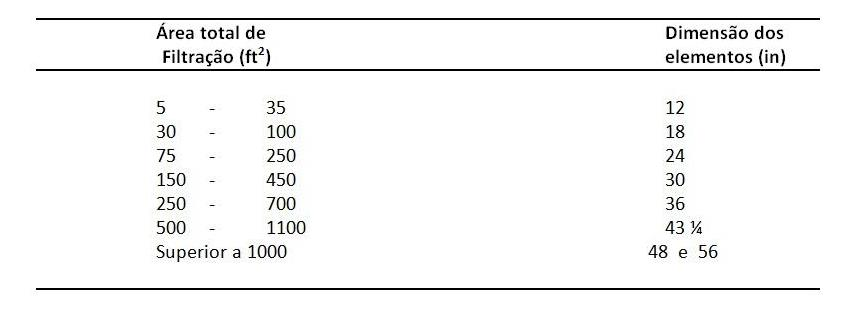
\includegraphics[scale=.6,trim={0 0 0 0}]{figuras/ladeq/filtra/tabquadro1}
		%\vspace{-20pt}
		\caption{Relação da área total de filtração com a dimensão dos quadros.}
		\label{tabqua1}
	\end{center}
\end{figure}



\begin{figure}[H]
	\begin{center}
		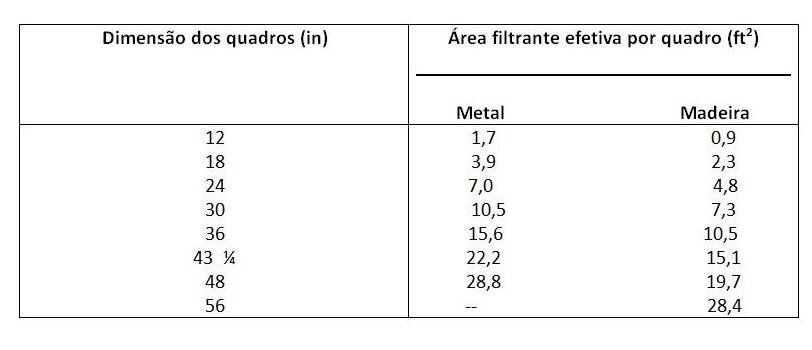
\includegraphics[scale=.6,trim={0 0 0 0}]{figuras/ladeq/filtra/tabquadro2}
		%\vspace{-20pt}
		\caption{Relação da dimensão dos quadros com a área efetiva de filtração de cada quadro, para quadros de madeira e de metal.}
		\label{tabqua2}
	\end{center}
\end{figure}

Foi escolhido o prato de dimensão igual a 30 in de metal, foi calculado então o número de pratos utilizados na operação industrial.



\begin{equation}\label{key}
N=\frac{213,213}{10,5}= 20,306 \approx 21 \ \text{quadros}
\end{equation}

\section{Projeto industrial do filtro-prensa}


Portanto, diante dos cálculos apresentados, para uma produção de filtrado de 13000 $ \dfrac{L}{h} $ de uma suspensão de carbonato de cálcio na concentração de $ 0,13269 \ \dfrac{g \ CaCO_{3}}{g \ \text{solução}}$ (PODE-SE COLOCAR EM FUNÇÃO H2O) com quadros de 1,2
in de espessura, o grupo propõe o seguinte projeto: 21 quadros de metal de dimensão 30 in e área total efetiva de 213,213 $ ft^{2} $.



\chapter{Conclusões}

%\chapter{Introdução}



\chapter{Apresentação das equações utilizadas}

\section{Filtração}


Para uma filtração sólido-líquido com formação de torta e considerando a torta como um meio poroso, aplica-se a equação do movimento para a torta:

\begin{tikzpicture}
\draw (0,0) node{$\displaystyle{
		\mathcal{L} \lbrace f(t)\rbrace = \int_{t=0}^\infty e^{-st} f(t)\,dt}$};
\end{tikzpicture}

\begin{equation}\label{key}
\rho\left[\varepsilon \frac{\partial \frac{q}{\varepsilon}}{\partial t}+\nabla\left(\frac{q}{\varepsilon}\right) q\right]=-\nabla P+\nabla \tau-m+\rho g
\end{equation}


onde:

\begin{itemize}

\item $\rho$ = densidade
\item $\varepsilon$ = porosidade da torta
\item q = velocidade superficial
\item P = pressão do sistema
\item $\tau$ = parâmetro proveniente de forças viscosas
\item g = aceleração da gravidade
\item m = massa de sólidos na torta

\end{itemize}

Suposições:

\begin{itemize}
\item Sem forças de campo;
\item Estado estacionário;
\item $\mathrm{\nabla\tau}= 0$ (sem interação viscosa);
\item Meio poroso isotrópico (k = cte.);
\item Escoamento a baixas velocidades ($Re_{MP}<1,0$)
\item Fluído;
\item Meio poroso rígido ($\varepsilon$ = cte.);
\item Meio poroso estacionário;
\item Escoamento isotérmico e incompressível ($\rho$=cte.);
\item Unidimensional e horizontal.
\end{itemize}

Então:

\begin{equation}\label{key}
\mathrm{m}=-\nabla P
\end{equation}

Com equação do movimento e a de  Darcy:

\begin{equation}\label{key}
\frac{d P}{d x}=\frac{\mu}{k} q
\end{equation}


E utilizando a definição de porosidade:

\begin{equation}\label{key}
\mathrm{dM}=\rho_{s}(1-\varepsilon) A d x
\end{equation}

Onde:

\begin{itemize}
\item $\mu$ = viscosidade do fluido;
\item A = área de filtração;
\item $\rho_{s}$ = densidade do sólido.
\end{itemize}

Fazendo as devidas substituições: e considerando PL = constante:

\begin{equation}\label{key}
d(P L-P)=\left(\frac{\mu q}{k \rho_{s}(1-\varepsilon) A}\right) d M
\end{equation}

A resistividade da torta ($\alpha$):

\begin{equation}\label{key}
\alpha=\frac{1}{k \rho_{s}(1-\varepsilon)}
\end{equation}

Logo,

\begin{equation}\label{key}
\mathrm{d}(\mathrm{PL}-\mathrm{P})=\left(\frac{\mu q a}{A}\right) d M
\end{equation}


\section{Dimensionamento Industrial}


Para o escalonamento de um filtro piloto para um filtro industrial consideramos que ambos operam com a mesma suspensão, a mesma queda de pressão e sob a mesma temperatura. Utilizando o subscrito ‘P’ para Piloto e ‘I’ para Industrial, temos as Equações \ref{DI1} e \ref{DI2} :

\begin{equation}\label{DI1}
V_{t P}=\frac{A_{P}}{2} e_{P}
\end{equation}

\begin{equation}\label{DI2}
V_{t I}=\frac{A_{I}}{2} e_{I}
\end{equation}


Em que, Vt é o volume da torta e  “e” a espessura do quadro. Considerando que o volume de torta é proporcional ao volume de filtrado (V) e combinando \ref{DI1}, \ref{DI2} à equação de trabalho, temos as Equações \ref{DI3} e \ref{DI4} :

\begin{equation}\label{DI3}
\frac{t_{P}}{t_{I}}=\frac{\left(\frac{V_{P}}{A_{P}}\right)^{2}}{\left(\frac{V_{I}}{A_{I}}\right)^{2}}
\end{equation}

\begin{equation}\label{DI4}
t_{I}=t_{P}\left(\frac{e_{I}}{e_{P}}\right)^{2}
\end{equation}


Com o tempo total de filtração na escala piloto, obtém-se o tempo total de filtração na escala industrial pela equação 13. Sabendo que o volume de filtrado industrial pode ser determinado pela Equação \ref{DI5}, da Equação \ref{DI3} calcula-se a área total de filtração industrial.

\begin{equation}\label{DI5}
V_{I}=P_{t} \cdot T_{I}
\end{equation}

Em que P é a vazão de produção da unidade industrial.
A vazão de produção de filtrado pode ser calculada como sendo a razão entre o volume de filtrado e o tempo total do ciclo de operação, incluindo o tempo de filtração , o tempo de lavagem dos quadros  e o tempo de montagem dos quadros  para a próxima operação, de acordo com a Equação \ref{DI6}. 

\begin{equation}\label{DI6}
P=\frac{V}{t_{f i l t}+t_{l a v}+t_{m o n t}}
\end{equation}


\chapter{Materiais e Métodos}

\section{Materiais}

\begin{itemize}

\item Suspensão de carbonato de cálcio;
\item Três vidros de relógio numerados;
\item Três becher numerados;
\item Duas provetas graduadas de 2L;
\item Um bastão de vidro;
\item Cronômetro (foi utilizado o cronômetro do celular de um dos integrantes do grupo);
\item Régua;
\item Espátula;
\item Filtro prensa (formado por dois quadros sem recheio, três placas rugosas e dois meios filtrantes);
\item Balança digital;
\item Estufa.


\end{itemize}

\section{Métodos}

Os bécher e vidros de relógio foram pesados e enumerados. Foram medidas as dimensões do quadro do filtro prensa com o auxilio de uma régua. 

O filtro prensa foi montado utilizando dois meios filtrantes. Estes foram umedecidos previamente para minimizar vazamentos. O filtro prensa utiliza dois quadros vazados que servem de suporte para os meios filtrantes e três placas rugosas. Durante a montagem do filtro prensa é realizada sobre o trilho do equipamento com placas e quadros intercalados de forme que duas placas fiquem nas extremidades. Foi verificada sistematicamente com uso de uma caneta se os furos de placas e quadros coincidem para que a suspensão possa para por todo o circuito do filtro-prensa. Após a verificação do ajuste do filtro, apertou-se o parafuso que mantem os quadros unidos e vedados contra o vazamento.

A solução de carbonato de cálcio presente no tanque de alimentação foi homogeneizada com auxílio de um bastão de vidro. \emph{Três amostras foram retiradas da suspensão} e pesadas nos bécher previamente pesados e identificados. Essa amostras foram então encaminhadas para uma estufa \emph{desligada durante cinco dias. No quinto dia a estufa foi ligada e. no sexto dia, as amostras secas foram pesadas novamente.}
 
Antes do início da filtração as provetas foram posicionadas de forma a coletar a solução filtrada e facilitar a troca rápida quando a primeira proveta chegar ao nível máximo. Com o tanque de alimentação já em recirculação, foi aberta a válvula a montante do filtro-prensa.

Com auxilo de provetas, o filtrado foi coletado. Durante este processo foram realizadas a marcação de volume filtrado em relação ao tempo de filtração. Para a marcação do tempo foi utilizado cronometro de celular operado por um dos alunos e com avisos sonoros dos alunos que operavam a coleta do filtrado na proveta.

A vazão de filtrado diminuiu durante a filtração e o experimento foi finalizado quando esta vazão ficou próxima de nula com a saída de gotas de filtrado. Foi coletado um total de 3,7 L de filtrado. A pressão de operação foi anotada e se manteve constante.


A torta formada nos quadros foi retirada e colocada sobre uma placa. Foram retiradas três alíquotas e alocadas em vidros de relógio já pesados e identificados. As amostras recolhidas nos vidros de relógio foram pesadas e mantidas na estufa desligada durante cinco dias. No quinto dia a estufa foi ligada e, no sexto dia, as amostras secas foram pesadas.

Ao final da prática, o filtrado e as tortas foram devolvidos ao tanque de alimentação.



\chapter{Resultados e Discussão}

\section{Propriedades Físicas}

Os dados apresentados na tabela a seguir foram obtidas do Manual de Engenharia Química, Perry and Chilton, 8a edição.

\begin{table}[H]
	\centering
	\begin{tabular}{|c|c|}
		\hline
		\rowcolor[HTML]{DAE8FC} 
		\textbf{Propriedade} & \textbf{Valor} \\ \hline
		Densidade da Água ($\rho F$) & $1,000 g \ \cdot cm^{-3}$ \\ \hline
		Viscosidade da Água ($\mu F$) & $1,00 \cdot E-3 \ Pa.s$ \\ \hline
		Densidade do Sólido ($\rho S$) & $2,711 \ g \cdot cm^{-3}$ \\ \hline
	\end{tabular}
	\caption{Propriedades Físicas da água e do sólido.}
	\label{tab:prop}
\end{table}


\section{Dados Experimentais}

\subsection{Cálculo da concentração em suspensão.}

A partir das massas da Tabela \ref{tab:massas}, calculou-se a concentração da suspensão da seguinte forma:

\begin{itemize}
	\item Massa da suspensão = (bécher + suspensão) - (bécher vazio)
	\item Massa seca = (bécher + massa seca) - (bécher vazio) 
	\item Concentração =  $\dfrac{\text{Massa de }CaCO_{3}}{\text{Massa da Suspensão}} $
\end{itemize}



\begin{table}[H]
	\centering
	\begin{tabular}{|c|c|c|c|}
		\hline
		\rowcolor[HTML]{DAE8FC} 
		\textbf{Bécher} & \textbf{Bécher vazio (g)} & \textbf{Bécher + suspensão (g)} & \textbf{Bécher  + sólido seco (g)} \\ \hline
		1 & 40,494 & 75,736 & 451,748 \\ \hline
		2 & 298,228 & 589,628 & 336,909 \\ \hline
		3 & 300,684 & 580,403 & 337,752 \\ \hline
	\end{tabular}
	\caption{Massas obtidas para o cálculo da concentração média da suspensão a ser filtrada.}
	\label{tab:massas}
\end{table}


As massas de sólido e de água foram calculadas para cada uma das três amostras e as concentrações obtidas estão apresentadas a seguir:

\begin{table}[H]
	\centering
	\begin{tabular}{|c|c|c|c|}
		\hline
		\rowcolor[HTML]{DAE8FC} 
		\textbf{Amostra} & \textbf{Massa de $CaCO_{3}$ (g)} & \textbf{Massa  da Suspensão (g)} & \textbf{Concentração $\frac{g CaCO_{3}}{g susp.}$} \\ \hline
		1 & 46,808 & 35,242 & 0,13282 \\ \hline
		2 & 38,681 & 29,14 & 0,13274 \\ \hline
		3 & 37,068 & 279,719 & 0,13252 \\ \hline
		\multicolumn{3}{|c|}{Média} & 0,13269 \\ \hline
	\end{tabular}
	\caption{Massas utilizadas no cálculo da concentração média da suspensão a ser filtrada.}
	\label{tab:massas2}
\end{table}

A concentração média obtida foi de 0,13269 $\dfrac{g \text{ de }  CaCO_{3}}{g \text{ de } susp.}$.


\subsection{Cálculo da porosidade média da torta}

\begin{table}[H]
	\centering
	\fontsize{10px}{10}\selectfont
	\begin{tabular}{|c|c|c|c|c|c|}
		\hline
		\rowcolor[HTML]{DAE8FC} 
		\textbf{\begin{tabular}[c]{@{}c@{}}Vidro de\\ Relógio\end{tabular}} & \textbf{\begin{tabular}[c]{@{}c@{}}Vidro de \\ Relógio vazio \\ (g)\end{tabular}} & \textbf{\begin{tabular}[c]{@{}c@{}}Vidro  de Relógio \\ + torta úmida\\ (g)\end{tabular}} & \textbf{\begin{tabular}[c]{@{}c@{}}Vidro de Relógio \\ + torta seca\\ (g)\end{tabular}} & \textbf{\begin{tabular}[c]{@{}c@{}}Torta Úmida\\ (g)\end{tabular}} & \textbf{\begin{tabular}[c]{@{}c@{}}Torta Seca \\ (g)\end{tabular}} \\ \hline
		1 & 343,432 & 514,536 & 449,302 & 171,104 & 105,870 \\ \hline
		2 & 44,149 & 594,163 & 529,781 & 152,673 & 88,291 \\ \hline
		3 & 367,894 & 532,342 & 462,667 & 164,448 & 94,773 \\ \hline
	\end{tabular}
	\caption{Massas dos vidros de relógio e tortas (g) obtidas para o cálculo da porosidade média da torta.}
	\label{tab:massas3}
\end{table}


Obtém-se o volume da água pela equação a seguir:

\begin{equation}\label{key}
V_{\text{água}} = \dfrac{M_{\text{água}}}{\rho_{\text{água}}}=\dfrac{M_{torta} - M_{\text{torta seca}}}{\rho_{\text{água}}}
\end{equation}

E o volume de torta seca:

\begin{equation}\label{key}
V_{\text { torta seca }}=\frac{M_{\text {torta seca}}}{\rho _{C a C O_{3}}}
\end{equation}

Por fim, obtém-se o Volume total por meio de:

\begin{equation}\label{key}
V_{total} = V_{\text{torta seca}}+V_{\texttt{água}} = M_{\texttt{torta seca}} + \dfrac{M_{torta} - M_{\texttt{torta seca}}}{\rho_{\text{água}}}
\end{equation}


Os resultados obtidos através dos cálculos demonstrados estão apresentados na Tabela \ref{tab:massas4}.


\begin{table}[H]
	\centering
		\begin{tabular}{|c|c|c|c|}
			\hline
			\rowcolor[HTML]{DAE8FC}
			\textbf{Amostra} & \textbf{\begin{tabular}[c]{@{}c@{}}Água\\ $(cm^{3})$ \end{tabular}} & \textbf{\begin{tabular}[c]{@{}c@{}}Torta seca\\ $(cm^{3})$ \end{tabular}} & \textbf{\begin{tabular}[c]{@{}c@{}}Torta Úmida \\ $(\text{Volume total - }cm^{3})$ \end{tabular}} \\ \hline
			1 & 6,5234 & 3,9052 & 10,4286 \\ \hline
			2 & 6,4382 & 3,2568 & 9,69497 \\ \hline
			3 & 6,9675 & 3,4959 & 10,46337 \\ \hline
	\end{tabular}
	\caption{Massas da torta úmida e seca.}
	\label{tab:massas4}
\end{table}




Por meio da Equação \ref{poro} foi possível determinar a porosidade média da torta:

\begin{equation}\label{poro}
\varepsilon = \dfrac{V_{\text{água}}}{V_{total}} = 1 - \dfrac{V_{\text{torta seca}}}{V_{total}}
\end{equation}

\begin{table}[H]
	\centering
	\begin{tabular}{|c|c|}
		\hline
		\rowcolor[HTML]{DAE8FC} 
		\textbf{Amostra} & \textbf{\begin{tabular}[c]{@{}c@{}}Porosidade\\   ($\varepsilon$)\end{tabular}} \\ \hline
		1 & 0,6255 \\ \hline
		2 & 0,6641 \\ \hline
		3 & 0,6659 \\ \hline
		Média & 0,6518 \\ \hline
	\end{tabular}
	\caption{Porosidade calculada para cada amostra e porosidade média.}
	\label{tab:poros}
\end{table}


Portanto, a porosidade média da torta é 0,6518.

\subsection{Cálculo da Resistividade da Torta ($\alpha$) e Resistência do Meio Filtrante ($R_m$)}

A resistividade da torta e a resistência do meio filtrante podem ser obtidos por meio do método gráfico no qual plota-se a curva t/V vs V a partir dos dados experimentais da filtração, apresentados na Tabela \ref{tab:corrida}.


\begin{table}[H]
	\centering
	\begin{tabular}{|c|c|c|}
		\hline
		\rowcolor[HTML]{DAE8FC} 
		\textbf{\begin{tabular}[c]{@{}c@{}}tempo \\ (s)\end{tabular}} & \textbf{\begin{tabular}[c]{@{}c@{}}Volume\\   Filtrado \\ (L)\end{tabular}} & \textbf{\begin{tabular}[c]{@{}c@{}}Tempo/Volume\\ (s/L)\end{tabular}} \\ \hline
		3,73 & 0,5 & 7,46 \\ \hline
		10,02 & 1 & 10,02 \\ \hline
		17,45 & 1,5 & 11,63 \\ \hline
		31,25 & 2 & 15,63 \\ \hline
		39,5 & 2,2 & 17,95 \\ \hline
		45,39 & 2,4 & 18,91 \\ \hline
		52,07 & 2,6 & 20,03 \\ \hline
		59,47 & 2,8 & 21,24 \\ \hline
		66,23 & 3 & 22,08 \\ \hline
		74,47 & 3,2 & 23,27 \\ \hline
		90,35 & 3,4 & 26,57 \\ \hline
		106,17 & 3,6 & 29,49 \\ \hline
		120,59 & 3,7 & 32,59 \\ \hline
	\end{tabular}
	\caption{Volume do filtrado (L) em função do tempo (s).}
	\label{tab:corrida}
\end{table}

Com os dados da tabela 7, plotou-se o gráfico a seguir:

\begin{figure}[H]
	\begin{center}
		\includegraphics[scale=1,trim={0 0 0 0}]{figuras/ladeq/filtra/graph1}
		%\vspace{-20pt}
		\caption{Curva de filtração - t/V (s/L) em função de V(L).}
		\label{apaTeo}
	\end{center}
\end{figure}

Os primeiros pontos não apresenta comportamento linear, pois no início do processo ainda não havia uma resistência significativa do meio filtrante e, por isso, a vazão de filtrado ainda era muito alta, obtendo-se assim, um grande volume de filtrado em um curto espaço de tempo, fazendo que a divisão tempo/volume ficasse muito baixo.

Por outro lado, no final do processo, a configuração exponencial do fim do gráfico indica que a torta estava completamente formada e não havia mais vazão de fluido. 

Diante do que foi dito anteriormente, para estimar os parâmetros de resistividade da torta e a resistência do meio filtrante, deve-se trabalhar apenas com a parte do gráfico que apresente comportamento linear. Sendo assim, os pontos iniciais e finais que fogem da linearidade foram desprezados.

\begin{figure}[H]
	\begin{center}
		\includegraphics[scale=1,trim={0 0 0 0}]{figuras/ladeq/filtra/graph2}
		%\vspace{-20pt}
		\caption{Curva de filtração - parte linear de t/V (s/L) em função de V(L).}
		\label{apaTeo}
	\end{center}
\end{figure}



Por fim, a  Resistividade da Torta $(\alpha)$ e Resistência do Meio Filtrante $(R_m)$, são obtidas por meio dos coeficientes angular e linear da equação obtida, de acordo com a equação a seguir:  


\begin{equation}\label{key}
\frac{t}{V}=\frac{\mu_{F}}{A \Delta p_{m}}\left(\frac{\alpha C p_{F} V}{2 A}+R_{m f}\right)
\end{equation}

Diante disso:

\begin{equation}\label{key}
\frac{t}{V}=5,2763 V+6,2747
\end{equation}

\begin{equation}\label{key}
\frac{\alpha \mu_{F} C p_{F}}{2 A^{2} \Delta p_{m}}=5,2763, \quad \frac{\mu_{F R_{m f}}}{A \Delta p_{m}}=6,2747
\end{equation}

A área de filtração pode ser obtida pela seguinte expressão: $A=2A_{P}2(0,9398)$, onde $A_{P}$ é a área de filtração na planta piloto $(A_{P}=16,2 \times16,3 cm^{2}=264,06 cm^{2} = 0,026406 m^{2}$ e 0,9298 é o fator de correção da placa. Desta forma, tem-se $A = 0,09927 m^{2}$.
O valor da queda de pressão foi mantido constante e igual a: $\Delta P= 5 kgf\cdot cm^{-2} = 49067,7 Pa$.
Em posse de todos os dados necessários para o cálculo da resistividade e resistência, basta isolar o $\alpha$ para encontrar o primeiro e o $R_{m}$ para o segundo:

\begin{equation}\label{key}
\alpha=5,2763 \frac{2 A^{2} \Delta p_{m}}{\mu_{F} C p_{F}}, R_{m f}=6,2747 \frac{A \Delta p_{m}}{\mu_{F}}
\end{equation}

\begin{equation}\label{key}
\alpha=3,8451 \times 10^{4} \ \mathrm{m} . \mathrm{kg}^{-1}, R_{m}=3,056 \times 10^{7} \ \mathrm{m}^{-1}
\end{equation}

\chapter{Dimensionamento Industrial}


\section{Dados}
Visando dimensionar um filtro industrial que atenda os seguintes parâmetros obtidos no procedimento experimental:



\begin{itemize}
\item Tempo de desmantelamento, lavagem e montagem do filtro: 20 minutos ou 1200 s (hipótese do grupo)
\item No roteiro diz para considerar $ t_{1} $ e $ t_{4} $ nulos!!!!!!!!!!!!
\item Tempo de filtração em escala piloto: 120,59 s;
\item Volume de filtrado em escala piloto: 3,7 L;
\item Espessura do quadro em escala piloto: 1,1 cm;
\item Pressão de filtração em escala piloto: $\Delta P= 49067,7 \ Pa$
\item Área de filtração em escala piloto: $ 0,026406 m^{2} $
\end{itemize}




Visando os seguintes parâmetros para a produção industrial:

\begin{itemize}
\item Pressão de filtração: Considerar mesma pressão da escala piloto.
\item Espessura do quadro em escala industrial: 3 cm 
\item Produção em escala industrial: 13000 $ \dfrac{L}{h} $ $ \approx 3,61 \ \dfrac{L}{s} $
\end{itemize}

\section{Determinação do tempo de filtração}


\begin{equation}\label{key}
\mathrm{t}_{\mathrm{IND}}=\mathrm{t}_{\mathrm{PIL}}\left(\frac{e_{I N D}}{e_{P I L}}\right)^{2}
\end{equation}


\begin{equation}\label{key}
t_{\mathrm{IND}}=120,59\left(\frac{3}{1,1}\right)^{2}=896,95\ s= 14,9491\ min \approx 15 \ min
\end{equation}

\section{Determinação do volume de filtrado industrial}




\begin{equation}\label{key}
\mathrm{P}_{\mathrm{IND}}=\frac{\mathrm{V}_{\mathrm{IND}}}{\mathrm{t}_{\mathrm{IND}}+t_{L}+t_{D}}
\end{equation}

\begin{equation}\label{key}
3,61=\frac{V_{I N D}}{896,95+1200}
\end{equation}


\begin{equation}\label{key}
\mathrm{V}_{\mathrm{IND}}=7572,321 \ L 
\end{equation}


\section{Determinação da área efetiva de filtração industrial}




\begin{equation}\label{key}
\mathrm{A}_{\mathrm{IND}}=\mathrm{A}_{\mathrm{PIL}} \frac{\mathrm{V}_{\mathrm{IND}}}{\mathrm{V}_{\mathrm{PIL}}} \frac{\mathrm{e}_{\mathrm{PIL}}}{\mathrm{e}_{\mathrm{IND}}}
\end{equation}

\begin{equation}\label{key}
\mathrm{A}_{\mathrm{IND}}=998,74 \frac{7572,321}{3,7} \cdot \frac{1,1}{3}=19,815 \ m^{2}
\end{equation}


\begin{equation}\label{key}
A_{\mathrm{IND}}=19,815 \ m^{2} \times 10,76 \ \frac{f t^{2}}{m^{2}}=213,213 \ f t^{2}
\end{equation}

A fim de propor um quadro específico para a área calculada, utilizou-se como base as tabelas abaixo:

\begin{figure}[H]
	\begin{center}
		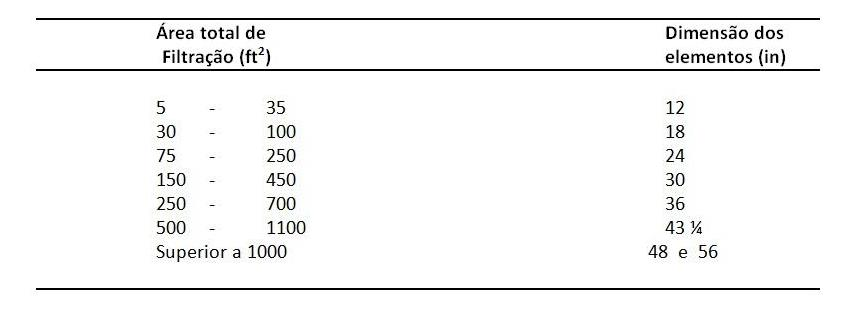
\includegraphics[scale=.6,trim={0 0 0 0}]{figuras/ladeq/filtra/tabquadro1}
		%\vspace{-20pt}
		\caption{Relação da área total de filtração com a dimensão dos quadros.}
		\label{tabqua1}
	\end{center}
\end{figure}



\begin{figure}[H]
	\begin{center}
		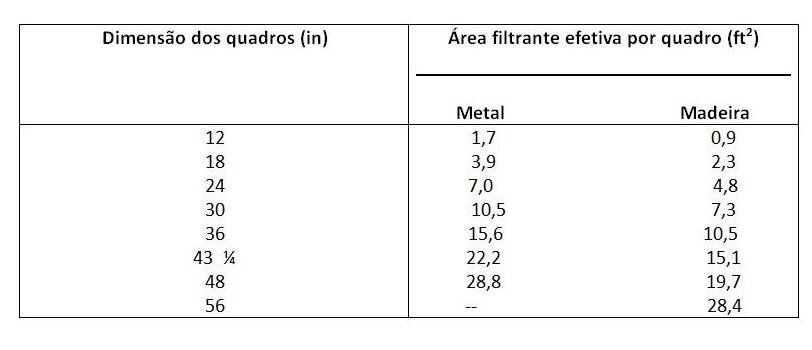
\includegraphics[scale=.6,trim={0 0 0 0}]{figuras/ladeq/filtra/tabquadro2}
		%\vspace{-20pt}
		\caption{Relação da dimensão dos quadros com a área efetiva de filtração de cada quadro, para quadros de madeira e de metal.}
		\label{tabqua2}
	\end{center}
\end{figure}

Foi escolhido o prato de dimensão igual a 30 in de metal, foi calculado então o número de pratos utilizados na operação industrial.



\begin{equation}\label{key}
N=\frac{213,213}{10,5}= 20,306 \approx 21 \ \text{quadros}
\end{equation}

\section{Projeto industrial do filtro-prensa}


Portanto, diante dos cálculos apresentados, para uma produção de filtrado de 13000 $ \dfrac{L}{h} $ de uma suspensão de carbonato de cálcio na concentração de $ 0,13269 \ \dfrac{g \ CaCO_{3}}{g \ \text{solução}}$ (PODE-SE COLOCAR EM FUNÇÃO H2O) com quadros de 1,2
in de espessura, o grupo propõe o seguinte projeto: 21 quadros de metal de dimensão 30 in e área total efetiva de 213,213 $ ft^{2} $.



\chapter{Conclusões}

\chapter{Introdução}



\chapter{Descrição Teórica do Sistema}


Para se projetar um sedimentador industrial é preciso determinar a área e a altura deste, com base no valor de concentração da alimentação e a concentração desejada na saída do sedimentador. Para isso, é necessário realizar testes de proveta para determinar alguns parâmetros em escala de laboratório.

Durante os testes de proveta, utiliza-se uma suspensão com as mesmas condições de temperatura e pH que são encontradas nos processo industrial. O teste de proveta permite obter a curva de posição da interface em função do tempo. A partir dessa curva, são obtidos parâmetros \emph{cinéticos} que permitem estimar a área e altura do sedimentador industrial.


\section{Etapas de Sedimentação e o teste da proveta}

Durante o processo de sedimentação, quatro zonas são formadas e nos testes de proveta realizados em escala de bancada, elas não são muito bem definidas.A fim de entender melhor como ocorre o mecanismo da sedimentação e como ela ocorre ao passar do tempo, pode-se analisar a Figura \ref{etapasprov}.


\begin{figure}[H]
	\begin{center}
		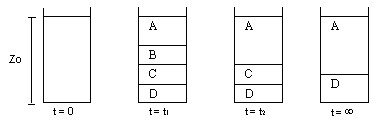
\includegraphics[scale=.8, trim={0 0 0 0}]{figuras/ladeq/sedi/proveta}
		%\vspace{-20pt}
		\caption{Mecanismo de sedimentação.}
		\label{etapasprov}
	\end{center}
\end{figure}


No início da decantação (t = 0), a suspensão encontra-se a uma altura $ Z_{0} $ e sua concentração é uniforme. Pouco tempo depois (t = $ t_{1} $ ) é possível distinguir quatro zonas distintas. São elas:


\begin{itemize}
\item A - Líquido Clarificado: esta camada pode ficar turva durante certo tempo devido à presença de partículas mais finas que permanecem em suspensão;
\item B - Região de Concentração constante ou concentração inicial: tem-se a sedimentação livre, isto é, desconsideram-se os efeitos de concentração, como se as partículas sedimentassem de forma isolada;
\item C - Região de Concentração Variável: nesta região a concentração da suspensão aumenta gradativamente, variando da concentração inicial até a concentração da suspensão espessada, e já se observa o efeito da concentração;
\item D - Região de Lama (compactação): à medida que ocorre a sedimentação a espessura desta região aumenta.  
\end{itemize}

À medida que a sedimentação ocorre, as regiões A e D tornam-se mais importantes e as regiões B e C tendem a desaparecer. 
A velocidade de sedimentação aumenta na região de clarificado (aceleração) e, a partir deste ponto, permanece constante até o final da região B. A velocidade tende a diminuir (desaceleração) em seguida até alcançar o ponto crítico de sedimentação, momento em que a região B desaparece \citep{macabe}.

Esse comportamento pode ser observado na Figura \ref{sedimentaP}.


\begin{figure}[H]
	\begin{center}
		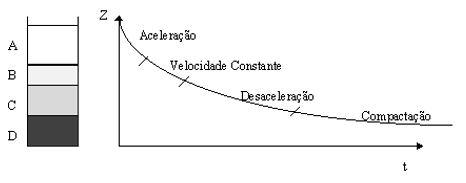
\includegraphics[scale=.8,trim={0 0 0 0}]{figuras/ladeq/sedi/graphProv}
		%\vspace{-20pt}
		\caption{Processo de Sedimentação.}
		\label{sedimentaP}
	\end{center}
\end{figure}

O ponto crítico pode ser determinado, pois enquanto a região B, de concentração igual à inicial, ainda existe, a velocidade de sedimentação é constante e, assim, a variação da altura da interface com o tempo é linear. Porém, ao B desaparecer, a velocidade de sedimentação começa a variar, devido ao fato da concentração também ser variável. Conforme a concentração aumentar, a velocidade de sedimentação diminui, como ilustrado na Figura \ref{linearReg}.


\begin{figure}[H]
	\begin{center}
		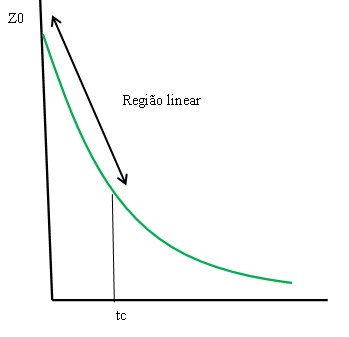
\includegraphics[scale=.5,trim={0 0 0 0}]{figuras/ladeq/sedi/graphProv2}
		%\vspace{-20pt}
		\caption{Determinação gráfica do tempo crítico (tC).}
		\label{linearReg}
	\end{center}
\end{figure}

\section{Balanço de Massa}

Um sedimentador, com suas respectivas correntes e concentrações, é representado no esquema da Figura \ref{esquema}.

\begin{figure}[H]
	\begin{center}
		\includegraphics[scale=.5,trim={0 0 0 0}]{figuras/ladeq/sedi/aparato}
		%\vspace{-20pt}
		\caption{Esquema de um sedimentador e suas variáveis.}
		\label{esquema}
	\end{center}
\end{figure}

Em que:

\begin{itemize}
\item Q – Vazão da alimentação
\item $ C_{v} $ – Concentração volumétrica de sólidos na alimentação
\item $ Q_{o} $ – Vazão volumétrica do overflow (líquido clarificado)
\item $ C_{vo} $ – Concentração volumétrica de sólidos no overflow
\item $ Q_{u} $ – Vazão volumétrica do underflow (sólidos concentrados, “lama”)
\item $ C_{vu }$ – Concentração volumétrica de sólidos no underflow
\item $ Q_{a} $ – Vazão volumétrica de líquido límpido no nível L em sentido ascendente
\item $ Q_{L} $ – Vazão volumétrica no nível L em sentido descendente
\item $ C_{vL} $ – Concentração de sólidos no nível L em sentido descendente
\end{itemize}



Para se iniciar o balanço de massa, considera-se que a concentração de sólidos na corrente de líquido clarificado é igual à zero. Logo, a vazão ascendente consiste apenas de líquido clarificado $ (C_{V0} = 0) $. Portanto, temos o seguinte balanço de massa para os sólidos:

\begin{equation}\label{key}
\rho s \times Q \times C v=\rho s \times Q u \times C v u=\rho s \times Q_{L} \times C v L
\end{equation}


Sendo $\rho_{S}$ a densidade das partículas sólidas. Portanto:

\begin{equation}\label{key}
\mathrm{Qu}=\mathrm{Q} \times \frac{\mathrm{Cv}}{\mathrm{Cvu}}
\end{equation}

Já para o líquido, temos o seguinte balanço de massa, no nível L:

\begin{equation}\label{key}
\rho \times \mathrm{Q}_{L} \times(1-\mathrm{CvL})=\rho \times \mathrm{Qa}+\rho \times \mathrm{Qu} \times(1-\mathrm{Cvu})
\end{equation}

Sendo $\rho$ a densidade do líquido. 
Assim,

\begin{equation}\label{key}
\mathrm{Qu}=\frac{\mathrm{Q}_{L} \times \mathrm{CvL}}{\mathrm{Cvu}}
\end{equation}

\begin{equation}\label{key}
Q_{L} \times(1-C v L)=Q a+\frac{Q_{L} \times C_{V L}}{C v u} \times(1-C v u)
\end{equation}

\begin{equation}\label{key}
\mathrm{Qa}=\mathrm{Q}_{L}-\mathrm{Q}_{L} \times \mathrm{CvL}-\frac{\mathrm{Q}_{L} \times \mathrm{CvL}}{\mathrm{Cvu}}+\mathrm{Q}_{L} \times \mathrm{CvL}
\end{equation}

\begin{equation}\label{key}
\mathrm{Q}_{L} \times \mathrm{CvL}=\mathrm{Q} \times \mathrm{Cv}
\end{equation}

\begin{equation}\label{key}
\mathrm{Qa}=\mathrm{Q}_{\mathrm{L}}-\frac{\mathrm{Q}_{L} \times \mathrm{CVL}}{\mathrm{Cvu}}=\mathrm{Q}_{L} \times \operatorname{CvL} \times\left(\frac{1}{\mathrm{CVL}}-\frac{1}{\mathrm{Cvu}}\right)
\end{equation}

\begin{equation}\label{key}
\mathrm{Qa}=\mathrm{Q} \times \mathrm{Cv} \times\left(\frac{1}{\mathrm{CvL}}-\frac{1}{\mathrm{Cvu}}\right)
\end{equation}

\begin{equation}\label{key}
\frac{\mathrm{Qa}}{\mathrm{A}}=\frac{\mathrm{Q} \times \mathrm{Cv}}{\mathrm{A}} \times\left(\frac{1}{\mathrm{CvL}}-\frac{1}{\mathrm{Cvu}}\right)
\end{equation}

A hipótese do método de Coe e Clevenger se baseia na sedimentação das partículas. Este método foi o primeiro a ser desenvolvido e é a fundamentação dos demais.Ele parte da ideia de que todas as partículas alimentadas devem seguir para zona de espessado. Caso isto não ocorra, acarretará no acúmulo de partículas, devido ao arraste, numa dada região chamada de zona limite.

Para tanto, tomando como base que $ C_{V0} = 0 $, a velocidade de ascensão do líquido deve ser menor que a velocidade de sedimentação das partículas, evitando, assim, que elas sejam arrastadas no sentido ascendente. Portanto, deve-se ter:



\begin{equation}\label{key}
\frac{\mathrm{Qa}}{\mathrm{A}} \leq \mathrm{v}
\end{equation}

Onde: $ \frac{Qa}{A} = $ velocidade de ascensão do fluido e v = velocidade de sedimentação das partículas.

No limite, tem-se:

\begin{equation}\label{key}
\frac{\mathrm{Qa}}{\mathrm{A}}=\mathrm{v}
\end{equation}

Assim:

\begin{equation}\label{key}
\frac{\mathrm{Q} \times \mathrm{Cv}}{\mathrm{A}} \times\left(\frac{1}{\mathrm{CvL}}-\frac{1}{\mathrm{Cvu}}\right)=\mathrm{v}
\end{equation}

Chegamos, então, à fórmula da área mínima:

\begin{equation}\label{key}
\mathrm{A}=\frac{\mathrm{Q} \times \mathrm{C} \mathrm{v}}{\mathrm{v}} \times\left(\frac{\mathrm{1}}{\mathrm{C} \mathrm{v} \mathrm{L}}-\frac{\mathrm{1}}{\mathrm{C} \mathrm{v} \mathrm{u}}\right)
\end{equation}


\section{Método de Kynch}

Kynch desenvolveu um método de dimensionamento de sedimentadores que necessita de apenas um ensaio experimental, diferentemente do método de Cloe e Clevenger, que exige inúmeros experimentos. 

O ensaio é iniciado com uma concentração uniforme $ C_{0} $. Supondo que, numa determinada seção do decantador, onde a concentração possui um valor C, a capacidade do equipamento passa por um mínimo e chega até um máximo quando o sistema está em operação, é nesse momento que uma zona característica começará a se formar nessa seção \citep{foust}. 

Se a seção transversal S for insuficiente,ocorrerá acúmulo de sólidos e a zona limite será deslocada para mais perto da saída de clarificado. Mas se a área for suficiente, em regime permanente, os sólidos que entram no sistema também saem.


O procedimento proposto por Kynch requer apenas um ensaio de decantação que forneça a curva de decantação (Z em função de t), através do qual se traçam tangentes em diversos pontos da curva e determinam-se os valores de t, Z e $ Z_{i} $. Com esses valores (t, Z e $ Z_{i} $), utiliza-se a expressão do método de Coe e Clevenger para obter as áreas da seção transversal.

O valor máximo de área obtida corresponderá à área mínima que o decantador poderá ter.

O método gráfico pode ser verificado na Figura \ref{met}.

\begin{figure}[H]
	\begin{center}
		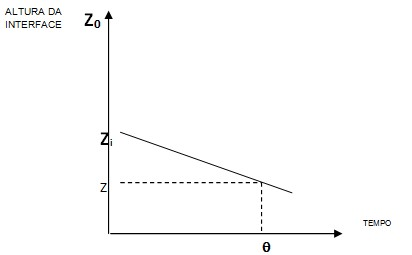
\includegraphics[scale=.5,trim={0 0 0 0}]{figuras/ladeq/sedi/graphKynch}
		%\vspace{-20pt}
		\caption{Exemplo de resultado do método de Kynch.}
		\label{met}
	\end{center}
\end{figure}


A reta tangente pode ser obtida após o cálculo de cada derivada, para cada altura da interface de sedimentação z, correspondente a um tempo de sedimentação t, utilizando as fórmulas a seguir:

\begin{equation}\label{key}
z=\frac{\mathrm{d} z}{\mathrm{dt}} \mathrm{t}+\mathrm{zi} \quad \quad \mathrm{zi}=z-\frac{\mathrm{d} z}{\mathrm{dt}} \mathrm{t}
\end{equation}

Assim, a concentração de sólidos em um nível L qualquer $ C_{vL} $ pode ser calculada, a partir dos valores de $ z_{i} $ correspondentes a cada altura da interface z, através da seguinte relação:

\begin{equation}\label{key}
\mathrm{C_{vL}}=\mathrm{C_{v}} \times \frac{\mathrm{z} _{0}}{\mathrm{z_{i}}}
\end{equation}

Finalmente, calcula-se a área mínima do sedimentador pela equação obtida pelo balanço de massa realizado acima:

\begin{equation}\label{key}
\operatorname{A_{min}}=\frac{\mathrm{Q} \times \mathrm{C_{v}}}{\mathrm{v}} \times\left(\frac{1}{\mathrm{C_{vL}}}-\frac{1}{\mathrm{C_{vU}}}\right)
\end{equation}

No final do experimento, tem-se um conjunto de áreas mínimas calculadas, que podem ser organizadas em uma tabela como a representada abaixo:

	

\begin{table}[H]
	\centering
	\begin{tabular}{|l|l|l|l|l|l|}
		\hline
		\textbf{t} & \textbf{z} & $ \mathbf{\left( \dfrac{d z}{dt}  \right)} $ & \textbf{zi} & $ \mathbf{C_{vL}} $ & \textbf{A} \\ \hline
		t1 & z1 & $ \left ( \dfrac{d z}{dt}\right )_{1} $ & zi1 & CvL1 & A1 \\ \hline
		t2 & z2 & $ \left ( \dfrac{d z}{dt} \right )_{2} $ & zi2 & CvL2 & A2 \\ \hline
		... & ... & ... & ... & ... & ... \\ \hline
		tn & zn & $ \left ( \dfrac{d z}{dt}\right )_{n} $ & zin & CvLn & An \\ \hline
	\end{tabular}
	\caption{Organização dos dados no método de Kynch.}
	\label{kynch}
\end{table}


Dentre todas as áreas mínimas calculadas pelo método de Kynch, a de maior valor deve ser utilizada como base de cálculo da área de projeto.


\section{Método de Biscaia Jr.}

Esse método é relativamente mais simples do que o método de Kynch. No método de Biscaia Jr., assume-se que a curva da altura da interface em função do tempo pode ser representada por uma função composta, sendo a primeira parte da curva linear e a segunda exponencial. 

$ Z_{\text{mín}} $ tem seu valor determinado a partir da seguinte relação:

\begin{equation}\label{key}
Z_{\min }=z_{0} * \frac{\mathrm{CvO}}{\mathrm{Cvu}}
\end{equation}

E com o valor de $ z_{\text{mín }}$, através do gráfico da Figura \ref{tabqua1}, obtém-se o valor de $ t_{\text{mín}} $.

\begin{figure}[H]
	\begin{center}
		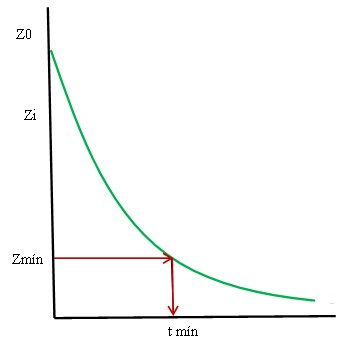
\includegraphics[scale=.5,trim={0 0 0 0}]{figuras/ladeq/sedi/graphBiscaia}
		%\vspace{-20pt}
		\caption{Representação gráfica do método de Biscaia Jr.}
		\label{tabqua1}
	\end{center}
\end{figure}


Com o valor detmín obtido, pode-se então determinar $ A_{\text{mín}} $:

\begin{equation}\label{key}
\operatorname{A_{\text{mín}}}=Q \times \frac{t_{\text{mín}}}{z_{0}}
\end{equation}


\section{Fatores de Correção}

A área determinada por ambos os métodos é a área mínima que o sedimentador deve ter para que se tenha a sedimentação desejada. Porém, é necessário o ajuste de alguns parâmetros para reproduzir as condições operacionais de um sedimentador industrial mais fielmente.


\begin{equation}\label{key}
A_{proj}=\operatorname{A_{\text{mín}}} \times \mathrm{f}_{1} \times \mathrm{f}_{2}
\end{equation}

O fator $ f_{1}  $considera efeitos de pH, temperatura, diâmetro dos flocos e concentração das partículas. Esse fator é especialmente importante em locais onde há grande variação de temperatura.

\begin{equation}\label{key}
1,10 \leq f_{1} \leq 1,25
\end{equation}


Já o fator $ f_{2} $ é função do diâmetro das partículas e considera a turbulência causada pela alimentação da suspensão no sedimentador. Como a velocidade nos tubos de alimentação é muito maior que a velocidade dentro do sedimentador, há geração de uma zona de turbulência na região de alimentação, dificultando a sedimentação. O fator de segurança visa amortecer o efeito da zona de turbulência através do aumento do diâmetro.

\begin{equation}\label{key}
1,10 \mathrm{m}<\mathrm{D}_{\mathrm{min}}<1,25 \mathrm{m} \quad 1,2 \leq \mathrm{f}_{2} \leq 1,5
\end{equation}

\begin{equation}\label{key}
D_{\min } \leq 5 \mathrm{m} \quad \mathrm{f}_{2}=1,5
\end{equation}

\begin{equation}\label{key}
\mathrm{D}_{\mathrm{min}} \geq 30 \mathrm{m} \quad \mathrm{f}_{2}=1,2
\end{equation}


\chapter{Objetivo}


O experimento tem como objetivo determinar o dimensionamento de um sedimentador a partir dos dados coletados em um teste de proveta para a suspensão de $ CaCO_{3} $, utilizando os métodos de Kynch e Biscaia Jr. e fazer comparações com os valores obtidos.

O sedimentador industrial deverá operar com uma suspensão de carbonato de cálcio, de aproximadamente 3\% em peso de $ CaCO_{3} $, para obtenção de uma lama de concentração de sólidos 2 vezes superior à da alimentação.
\\


\chapter{Materiais e Métodos}

\section{Materiais}

\begin{itemize}
\item Suspensão de carbonato de cálcio;
\item 1 Proveta graduada de 2L;
\item 3 Vidros de relógio;
\item Pipeta;
\item Bastão de Vidro;
\item Balança analítica digital;
\item Cronômetro;
\item Tira de papel milimetrado;
\item Estufa.
\end{itemize}

\section{Métodos}

Realizou-se o teste de proveta usando 2 L da suspensão de carbonato de cálcio. Para determinar a concentração real da suspensão, antes do início do teste, colocou-se 3 amostras em vidros de relógios secos previamente pesados. Após a adição da suspensão, os vidros foram novamente pesados. As amostras foram à estufa por, aproximadamente, $ 100^{\circ} $C até peso constante e então novamente os vidros foram pesados.


O teste de proveta iniciou assim que os 2L de solução estavam bem homogeneizados na proveta, com o auxílio do bastão de vidro, iniciando o cronômetro. A sedimentação iniciou e foi possível observar a formação de 2 fases, uma mais opaca com alto teor de sólidos e uma clarificada. A interface foi monitorada e o tempo anotado a cada decréscimo da mesma em 0,5 cm de altura. Com os pontos, foi possível plotar o gráfico $ Z \times t $.




\chapter{Resultados e Discussão}

\section{Propriedades físico-químicas}

\begin{itemize}
\item Densidade da água$  (\rho): 1 \ \dfrac{g}{cm^{3}} $
\item Densidade do carbonato de cálcio $ (\rho _{S}): 2,711 \ \dfrac{g}{cm^{3}} $ (a $ 25^{\circ} $C)
\item Viscosidade da água $ (\mu): 0,01 \ \dfrac{g \cdot cm}{s}$ 
\end{itemize}




\section{Determinação da concentração e densidade de $ \mathbf{CaCO_{3}} $ na suspensão}


Para determinação das concentrações mássica e volumétrica, utilizaram-se os dados da Tabela \ref{param}.

\begin{table}[H]
	\centering
	\begin{tabular}{|c|c|c|c|}
		\hline
		\textbf{Numeração} & \textbf{\begin{tabular}[c]{@{}c@{}}M1: Vidro de relógio\\  vazio (g)\end{tabular}} & \textbf{\begin{tabular}[c]{@{}c@{}}M2: Vidro de relógio \\ com suspensão inicial (g)\end{tabular}} & \textbf{\begin{tabular}[c]{@{}c@{}}M3: Vidro de relógio \\ com suspensão seca (g)\end{tabular}} \\ \hline
		S1 & 36,0549 &  & 39,1954 \\ \hline
		S2 & 44,723 &  & 44,8572 \\ \hline
		S3 & 36,0498 &  & 36,1928 \\ \hline
	\end{tabular}
	\caption{Tabela com as massas em cada etapa do procedimento.}
	\label{param}
\end{table}

A partir dos resultados experimentais, os cálculos realizados foram: $ H_{2}O $ e $ CaCO_{3} $ foram determinados do seguinte modo:


\begin{itemize}
\item Massa de $ H_{2}O: M_{2} – M_{3} $
\item Massa de $ CaCO_{3}: M_{3}-M_{1} $
\item Volume de $ H_{2}O $: $\dfrac{(M_{2} – M_{3})}{\rho}$
\item Volume de $ CaCO_{3} $:  $\dfrac{(M_{3}-M_{1})}{\rho_{S}}$
\end{itemize}

\subsection{Cálculos}

Determinar a concentração mássica significa efetuar a seguinte razão:
\begin{equation}\label{key}
\mathrm{C}_{m}=\frac{\text { massa de sólido }\left(\mathrm{CaCO}_{3}\right)}{\text { massa de suspensão }}=\frac{\text { massa de sólido }\left(\mathrm{CaCO}_{3}\right)}{\text { massa de água }+\text { massa de } \mathrm{CaCO}_{3}}
\end{equation}


Determinar a concentração volumétrica significa efetuar:

\begin{equation}\label{key}
C_{V}=\frac{ V_{\text{sólido}} \left(\mathrm{CaCO}_{3}\right)}{V_{\text{suspensão}}}
\end{equation}


\begin{equation}\label{key}
\mathrm{V}_{ \text {sólido}}=\frac{\text { massa sólidos }\left(\mathrm{CaCO}_{3}\right)}{\rho_{S}}
\end{equation}


\begin{equation}\label{key}
V_{\text{suspensão}} = V_{\text{água}}+V_{\text{sólidos}}
\end{equation}


\begin{equation}\label{key}
V_{\text{suspensão}} = \dfrac{ \text{massa água} }{\rho}+\dfrac{\text { massa sólidos (CaCO }_{3} )}{\rho_{s}}
\end{equation}


\begin{equation}\label{key}
\mathrm{C}_{V}=\frac{\frac{\text { massa sólidos }}{\rho_{S}}}{\frac{\text { massa água }}{\rho}+\frac{\text { massa sólidos }}{\rho_{S}}}
\end{equation}

Determinar a densidade da suspensão significa efetuar:

\begin{equation}\label{key}
\rho_{\text { suspensäo }}=\frac{\text { massa suspensão }}{\mathrm{V} \text { suspensão }}
\end{equation}

\begin{equation}\label{key}
\rho_{\text { suspensão }}=\frac{\text { massa suspensão }}{\text { volume } \mathrm{CaCO}_{3}+\text { volume } \mathrm{H_{2} O}}
\end{equation}


\begin{equation}\label{key}
\rho_{\text { suspensão }}=\frac{\text { massa suspensão }}{\frac{\text { massa }CaCO_{3}}{\rho_{S}}+\frac{\text { massa } \mathrm{H_{2} O}}{\rho}}
\end{equation}

\begin{table}[H]
	\centering
	\begin{tabular}{|c|c|c|c|c|}
		\hline
		\textbf{Numeração} & \textbf{\begin{tabular}[c]{@{}c@{}}Massa de água \\ (g)\end{tabular}} & \textbf{\begin{tabular}[c]{@{}c@{}}Massa de CaCO3 \\ (g)\end{tabular}} & \textbf{\begin{tabular}[c]{@{}c@{}}Volume de água \\ (mL)\end{tabular}} & \textbf{\begin{tabular}[c]{@{}c@{}}Volume de CaCO3 \\ (mL)\end{tabular}} \\ \hline
		S1 &  & 3,1405 &  &  \\ \hline
		S2 &  & 0,1342 &  &  \\ \hline
		S3 &  & 0,143 &  &  \\ \hline
	\end{tabular}
	\caption{Cálculos do volume de água e de sólido.}
	\label{vol}
\end{table}


\begin{table}[H]
	\centering
	\begin{tabular}{|c|c|c|c|}
		\hline
		\textbf{Numeração} & \textbf{\begin{tabular}[c]{@{}c@{}}Concentração\\   Volumétrica (\%v/v)\end{tabular}} & \textbf{\begin{tabular}[c]{@{}c@{}}Concentração\\   Mássica (\%m/m)\end{tabular}} & \textbf{\begin{tabular}[c]{@{}c@{}}Densidade\\   da Suspensão (g/cm³)\end{tabular}} \\ \hline
		S1 &  &  &  \\ \hline
		S2 &  &  &  \\ \hline
		S3 &  &  &  \\ \hline
		Média &  &  &  \\ \hline
	\end{tabular}
	\caption{Cálculos das concentrações de sólido.}
	\label{tab:my-table}
\end{table}

\section{Teste de Proveta}

\subsection{Altura inicial da proveta}

Sabendo-se que a $ \text{Área} = \dfrac{\pi D^{2}}{4} $ e $ Volume = \text{Área} \cdot Z_{0} $, temos:

\begin{table}[H]
	\centering
	\begin{tabular}{|c|c|}
		\hline
		\textbf{\begin{tabular}[c]{@{}c@{}}Diâmetro da proveta\\  (cm)\end{tabular}} & 8,1 \\ \hline
		\textbf{\begin{tabular}[c]{@{}c@{}}Área da seção transversal \\ da proveta (cm²)\end{tabular}} & 51,53 \\ \hline
		\textbf{\begin{tabular}[c]{@{}c@{}}Volume inicial \\     (cm³ = mL)\end{tabular}} & 2000 \\ \hline
		\textbf{\begin{tabular}[c]{@{}c@{}}Altura inicial \\ de líquido (cm)\end{tabular}} & 38,81 \\ \hline
	\end{tabular}
	\caption{Dados do sistema montado para o teste de proveta.}
	\label{dadosprov}
\end{table}


\subsection{Curva de sedimentação (altura da proveta x tempo)}

Uma vez iniciada a sedimentação, o grupo anotou o tempo para a suspensão sedimentar a cada 0,5 cm, obtendo a seguinte curva:


Diante da curva apresentada, efetuaram-se dois ajustes, um linear, inicialmente, e um exponencial. Considerou-se adequado, uma vez que os coeficientes de correlação estão próximos a 1. Com as equações ajustadas, utilizaram-se os métodos para determinação da área do sedimentador. 

\subsection{Método de Kynch}

Segundo o método de Kynch, a área mínima do sedimentador pode ser calculada pela equação abaixo:

\begin{equation}\label{key}
\mathrm{A} \min =\frac{\mathrm{Q} * \mathrm{C}_{V}}{\mathrm{v}} *\left(\frac{1}{\mathrm{C}_{V L}}-\frac{1}{\mathrm{C}_{V U}}\right)
\end{equation}

Onde:

\begin{itemize}
	\item $ \mathrm{Q}=\frac{\text { Qmássica }}{\text { Psuspensäo }} $;
	\item $ C_{v}  $ Concentração volumétrica de alimentação;
	\item $ v=\frac{-d z}{d t} $
	\item $ \mathrm{C}_{V L}=\mathrm{C}_{V} * \frac{\mathrm{z}_{0}}{\mathrm{z}_{I}} $
	\item $ \mathrm{z}_{I}=\mathrm{z}-\frac{\mathrm{d} z}{\mathrm{dt}} * \mathrm{t} $
	\item 
\end{itemize}

\subsubsection{Tabela com os valores calculados para área}


\subsubsection{Fatores de correção}


\subsubsection{Projeto de sedimentador}

\subsection{Método de Biscaia Jr.}

\subsubsection{Determinação de $ \mathbf{Z_{\text{mín}}} $ e $ \mathbf{t_{\text{mín}}} $}


\begin{equation}\label{key}
Z_{\text{mín}} =\mathrm{Z}_{0} * \frac{\mathrm{C}_{V 0}}{\mathrm{C}_{V U}}
\end{equation}


\subsubsection{Determinação de $ A_{\text{mín}} $}

\begin{equation}\label{key}
A_{m i n}=Q * \frac{t_{m \hat{m}}}{Z_{0}}
\end{equation}

\subsubsection{Fatores de correção}

\subsubsection{Projeto do sedimentador}

\subsection{Comparação entre os métodos}

\chapter{Conclusões}

%\include{chapters/ladeq/CINETICA}







\newpage 
%style{custom}
%\bibliographystyle{plainnat}
\bibliographystyle{achemso}
%\bibliographystyle{rsc}




%________________BIBLIOGRAFIAS

\bibliography{bib/SEDIMENTA}
%\bibliography{bib/DIFUSAO}






\end{document}